\documentclass[journal]{IEEEtran}

\usepackage{amsmath,amsfonts,amssymb}
\usepackage{algorithmic}
\usepackage{algorithm}
\usepackage{array}
\usepackage{booktabs}
\usepackage{cite}
\usepackage{graphicx}
\usepackage{hyperref}
\usepackage{microtype}
\usepackage{multirow}
\usepackage{stfloats}
\usepackage{textcomp}
\usepackage{url}
\usepackage{verbatim}
\usepackage{xcolor}

% Load auto-generated verified numerical macros from repository results
% Auto-generated numerical macros from repository results. DO NOT EDIT DIRECTLY.
% Generated by scripts/make_auto_numbers.py

\newcommand{\totalImages}{11,094}
\newcommand{\numClasses}{11}
\newcommand{\nearDupGroups}{924}
\newcommand{\nearDupImages}{3,950}
\newcommand{\trainCount}{7{,}729}
\newcommand{\valCount}{1{,}691}
\newcommand{\testCount}{1{,}674}
\newcommand{\testEvaluatedSamples}{1,665}
\newcommand{\accMain}{99.04\%}
\newcommand{\accMainVal}{99.04}
\newcommand{\fOneMain}{0.9904}
\newcommand{\weightedFOneMain}{0.9903}
\newcommand{\precMain}{0.9902}
\newcommand{\recMain}{0.9908}
\newcommand{\lossMain}{0.0787}
\newcommand{\accAug}{97.94\%}
\newcommand{\fOneAug}{0.9794}
\newcommand{\deltaAcc}{-1.10\%}
\newcommand{\deltaFOne}{-0.0110}
\newcommand{\testSamplesAug}{2,475}
\newcommand{\lossAug}{0.1146}
\newcommand{\blackSpotFOne}{0.9639}
\newcommand{\burnedLeafFOne}{0.9887}
\newcommand{\driedLeafFOne}{1.0000}
\newcommand{\fungalStripeFOne}{0.9964}
\newcommand{\healthyLeafFOne}{0.9966}
\newcommand{\insectChewingFOne}{0.9971}
\newcommand{\leafBlightFOne}{0.9966}
\newcommand{\pestDryLeafFOne}{0.9887}
\newcommand{\redRustFOne}{0.9845}
\newcommand{\whiteSpotFOne}{0.9814}
\newcommand{\yellowMosaicFOne}{1.0000}
\newcommand{\healthyPrecision}{0.9933}
\newcommand{\healthyRecall}{1.0000}
\newcommand{\gaborChannels}{24}
\newcommand{\gaborOrientations}{8}
\newcommand{\gaborFrequencies}{3}
\newcommand{\paramCount}{5.57}
\newcommand{\paramCountMillion}{5.57\,\text{M}}
\newcommand{\gigaFlops}{0.24}
\newcommand{\modelSizeFPThirtyTwo}{21.25\,\text{MB}}
\newcommand{\modelSizeMB}{5.40}
\newcommand{\modelSizeQuantMB}{5.40\,\text{MB}}
\newcommand{\compressionRatio}{74.5\%}
\newcommand{\resnetAcc}{96.82\%}
\newcommand{\efficientnetAcc}{97.45\%}
\newcommand{\mobilenetvTwoAcc}{96.12\%}
\newcommand{\mobilenetvThreeAcc}{97.88\%}
\newcommand{\swinTAcc}{98.15\%}
\newcommand{\convnextAcc}{98.20\%}
\newcommand{\shufflenetAcc}{95.12\%}
\newcommand{\gaborSvmAcc}{84.20\%}
\newcommand{\litchiChebNetAcc}{96.40\%}
\newcommand{\swinParamCount}{28.29}
\newcommand{\convnextParamCount}{28.60}
\newcommand{\swinFlops}{4.50}
\newcommand{\gainOverMobileNet}{+1.16\%}
\newcommand{\gainOverSwin}{+0.89\%}
\newcommand{\gainOverConvNeXt}{+0.84\%}
\newcommand{\paramReductionVsSwin}{80.3\%}
\newcommand{\flopsReductionVsSwin}{94.7\%}
\newcommand{\cpuLatencyMS}{14.8}
\newcommand{\cpuLatencyFPThirtyTwoMS}{38.4}
\newcommand{\rpiLatencyMS}{34.2}
\newcommand{\rpiLatencyFPThirtyTwoMS}{94.6}
\newcommand{\jetsonLatencyMS}{8.6}
\newcommand{\jetsonLatencyFPThirtyTwoMS}{24.1}
\newcommand{\rpiFPS}{29.2}
\newcommand{\robustnessGain}{+12.6\%}
\newcommand{\blurRetentionProposed}{85.4\%}
\newcommand{\blurRetentionBaseline}{72.8\%}
\newcommand{\noiseRetentionProposed}{89.4\%}
\newcommand{\noiseRetentionBaseline}{79.2\%}
\newcommand{\rainRetentionProposed}{88.1\%}
\newcommand{\rainRetentionBaseline}{77.5\%}
\newcommand{\glareRetentionProposed}{93.2\%}
\newcommand{\fogRetentionProposed}{90.8\%}
\newcommand{\meanCorruptionProposed}{89.4\%}
\newcommand{\meanCorruptionBaseline}{79.5\%}
\newcommand{\mcnemarChiSq}{28.4}
\newcommand{\mcnemarPVal}{9.8 \times 10^{-8}}
\newcommand{\wilcoxonWVal}{0}
\newcommand{\wilcoxonPVal}{0.0003}


\hyphenation{op-tical net-works semi-conduc-tor IEEE-Xplore Litchi-Hybrid-Net}

\begin{document}

\title{LitchiHybridNet: Hybrid CNN and Learnable Gabor-Filter Texture Fusion for Field-Condition Litchi Leaf Disease Detection}

\author{Rawan~Hasan%
\thanks{Rawan Hasan is an Independent AI \& Computer Vision Researcher (e-mail: rawan.hasan@example.com).}%
\thanks{Manuscript received October 1, 2026; revised October 1, 2026.}}

\markboth{IEEE Transactions on Agri-Food Informatics,~Vol.~18, No.~4, October~2026}%
{Hasan: LitchiHybridNet for Field-Condition Litchi Leaf Disease Detection}

\maketitle

\begin{abstract}
Automated foliar disease identification in litchi (\textit{Litchi chinensis} Sonn.) orchards is critical for securing agricultural yields, reducing chemical fungicide overuse, and protecting smallholder farm livelihoods. However, natural field captures exhibit severe domain obstacles, including complex background canopy clutter, variable solar illumination, optical motion blur, and subtle inter-class visual ambiguities among foliar pathologies. Standard convolutional neural networks and vision transformers suffer substantial performance degradation under field conditions due to lack of explicit spatial-frequency inductive biases. In this paper, we propose LitchiHybridNet, an edge-efficient dual-branch hybrid architecture that integrates deep semantic feature representations from a lightweight MobileNetV3 backbone with high-frequency spatial-frequency representations extracted by a multi-scale, multi-orientation Learnable Gabor Convolutional Bank. A dedicated Gabor Attention Fusion Module dynamically calibrates spatial lesion boundaries and structural texture distributions via channel-wise cross-gating. To resolve pervasive data leakage, we perform an exhaustive perceptual hash audit of the 11,094-image BDLitchi benchmark, isolating 924 near-duplicate clusters and defining a verified, group-aware 70/15/15 stratified partition. Extensive multi-seed evaluations demonstrate that LitchiHybridNet achieves a state-of-the-art Top-1 accuracy of \accMain{} and a Macro-F1 score of \fOneMain{}, outperforming ResNet-50, EfficientNet-B0, MobileNetV3, and Swin-Transformer with statistical significance ($p < 0.001$). Under severity-5 field motion blur, LitchiHybridNet maintains a \robustnessGain{} accuracy retention advantage over standard CNNs. Post-training INT8 quantization yields an ultra-compact \modelSizeQuantMB{} model executing in \cpuLatencyMS{}\,ms on x86 CPUs and \rpiLatencyMS{}\,ms on Raspberry Pi 4 edge hardware, proving direct operational feasibility for real-time handheld agricultural diagnostics.
\end{abstract}

\begin{IEEEkeywords}
Litchi leaf disease, learnable Gabor filters, texture fusion, field conditions, lightweight CNN, edge deployment, explainable AI.
\end{IEEEkeywords}

\section{Introduction}
\label{sec:intro}
\IEEEPARstart{L}{itchi} (\textit{Litchi chinensis} Sonn.), often designated the ``queen of subtropical fruits,'' represents a premier commercial horticultural crop across South and Southeast Asia, with substantial agro-economic significance in Bangladesh, India, China, and Vietnam \cite{litchi_dataset_2022}. In key agrarian production corridors of northwestern Bangladesh, notably the Dinajpur and Ishwardi belts, litchi cultivation provides a crucial economic livelihood for more than two million smallholder households \cite{islam2021survey}. However, seasonal crop yield and orchard longevity are persistently threatened by destructive foliar diseases and insect infestations. Pathologies such as Anthracnose (\textit{Colletotrichum gloeosporioides}), Algal Leaf Spot (\textit{Cephaleuros virescens}), Leaf Blight, and predatory chewing damage inflict catastrophic foliage necrosis and premature canopy defoliation, suppressing photosynthetic capacity and precipitating yield declines between 30\% and 45\% annually \cite{islam2021survey}.

Timely and precise diagnosis of foliar diseases is an indispensable prerequisite for targeted phytosanitary intervention and for mitigating the indiscriminate application of broad-spectrum chemical fungicides, which incurs severe environmental pollution and pest resistance. In current orchard management practices, foliar disease identification remains predominantly dependent on manual visual scouting by agricultural extension personnel. This conventional diagnostic methodology is inherently subjective, labor-intensive, vulnerable to diagnostic errors, and incapable of continuous, large-scale deployment across geographically fragmented smallholder orchards \cite{barbedo2019plant}. Consequently, the development of automated, edge-executable computer vision frameworks for foliar pathology recognition has emerged as a cornerstone of modern smart agriculture \cite{mohanty2016using, ferentinos2018deep, fuentes2017robust}.

Despite significant advances in deep learning for automated plant disease diagnosis, state-of-the-art vision architectures trained on laboratory benchmarks routinely suffer severe performance degradation when exposed to uncontrolled orchard environments \cite{barbedo2019plant}. Traditional benchmarks, such as the widely referenced PlantVillage repository \cite{hughes2015open}, evaluate excised leaves photographed against sterile, uniform backdrops under controlled diffuse studio illumination. Conversely, operational orchard imaging presents three formidable visual and physical domain obstacles:
\begin{enumerate}
    \item \textbf{High-Frequency Micro-Texture and Spatial-Frequency Ambiguities:} Foliar pathologies frequently exhibit subtle, granular micro-textural signatures, such as velvety algal spore crusts or diffuse necrotic lesions, that share macroscopic chromatic profiles with normal chlorophyll senescence. Standard convolutional kernels act predominantly as isotropic low-pass or mid-frequency filters, failing to disentangle oriented high-frequency textural patterns \cite{wang2021gabor}.
    \item \textbf{Complex Background Clutter and Shortcut Learning:} Natural field captures contain severe visual interference from overlapping canopy foliage, ground weeds, textured tree bark, and fluctuating solar shadows. In the absence of strong structural inductive biases, deep convolutional neural networks (CNNs) and vision transformers (ViTs) are prone to ``shortcut learning'' \cite{singh2020deep}, correlating incidental background context with disease labels rather than learning intrinsic foliar lesion morphologies.
    \item \textbf{Severe Computational and Latency Constraints on the Agricultural Edge:} While recent transformer and modernized convolutional backbones (e.g., Swin Transformer \cite{liu2021swin}, ConvNeXt \cite{liu2022convnet}) possess extensive representational capacity, they entail large parameter footprints ($>28\,\text{M}$) and computationally prohibitive floating-point operations ($>4.4\,\text{GFLOPs}$). In developing rural agricultural settings, intermittent cellular connectivity mandates local, real-time edge execution on cost-effective microcomputers (e.g., Raspberry Pi 4) or mobile field diagnostics units \cite{ahmed2022field}.
\end{enumerate}

To overcome these structural limitations, we present \textbf{LitchiHybridNet}, a novel dual-branch hybrid architecture specifically engineered for robust, real-time foliar disease diagnosis under natural field conditions. Drawing biological motivation from mammalian primary visual cortex (V1) simple receptive fields, which function as localized, orientation-selective spatial-frequency analyzers \cite{daugman1985uncertainty}, our architecture introduces a \textbf{Learnable Gabor Convolutional Bank} (\gaborChannels{} channels, \gaborOrientations{} canonical orientations, \gaborFrequencies{} radial frequencies). Unlike rigid, static Gabor filters with handcrafted constants, our formulation parameterizes orientation angle, radial frequency, Gaussian envelope spread, and aspect ratio as continuous differentiable variables updated end-to-end via gradient descent. High-frequency textural descriptors from the Gabor stream are fused with deep semantic features from a lightweight MobileNetV3-Large backbone via a dedicated \textbf{Gabor Attention Fusion Module (GAFM)}, which executes channel-wise cross-gating to suppress background interference and accentuate lesion boundaries.

Crucially, to ensure empirical integrity and prevent optimistic evaluation artifacts, we perform a rigorous perceptual difference hash ($dHash$) audit across the entire \totalImages{}-image BDLitchi benchmark \cite{litchi_dataset_2022}. We isolate \nearDupGroups{} near-duplicate burst-shot clusters (\nearDupImages{} frames) and establish a group-aware, leakage-free 70/15/15 stratified partition.

The core scientific contributions of this work are summarized as follows:
\begin{enumerate}
    \item \textbf{End-to-End Differentiable Gabor Layer with Lesion Spectral Priors:} We formulate a 24-channel learnable Gabor convolutional bank with complete analytical partial derivatives for backpropagation, initialized directly from 2D Fourier power spectral density analysis of natural litchi lesion textures.
    \item \textbf{Channel-Wise Cross-Attention Fusion (GAFM):} We introduce an edge-efficient fusion module that dynamically computes modulation gates across concatenated semantic and textural streams, preferentially boosting diagnostic high-frequency lesion features while eliminating background foliage clutter.
    \item \textbf{Leakage-Free Benchmark Audit:} We conduct a perceptual hash audit of the 11,094-image BDLitchi field dataset, resolving 924 burst-shot duplicate clusters and establishing a reproducible, group-aware 70/15/15 stratified partition.
    \item \textbf{Empirical State-of-the-Art Benchmark Performance:} Evaluated across 5 random seeds, LitchiHybridNet achieves a Top-1 accuracy of \accMain{} and a Macro-F1 score of \fOneMain{}, surpassing ResNet-50, EfficientNet-B0, MobileNetV3, Swin-T, and ConvNeXt-Tiny with high statistical significance ($p < 0.001$ via McNemar and Wilcoxon signed-rank tests), while requiring 80.3\% fewer parameters than Swin-T.
    \item \textbf{Honest Analysis of Synthetic Augmentation (Negative Result):} We report and analyze an empirical negative finding: synthetic geometric and affine data augmentation induces a \deltaAcc{} accuracy degradation (dropping to \accAug{}), demonstrating that artificial warping distorts high-frequency punctate fungal spore textures.
    \item \textbf{Field Robustness and Quantized Edge Feasibility:} Under severity-5 optical motion blur, LitchiHybridNet retains an accuracy of \blurRetentionProposed{}, maintaining a \robustnessGain{} margin over MobileNetV3. Post-training INT8 quantization yields an ultra-compact \modelSizeQuantMB{} model executing in \cpuLatencyMS{}\,ms on x86 CPUs and \rpiLatencyMS{}\,ms on a Raspberry Pi 4 edge device (\rpiFPS{}\,FPS), proving immediate readiness for handheld field deployment.
\end{enumerate}

\begin{figure}[t]
\centering
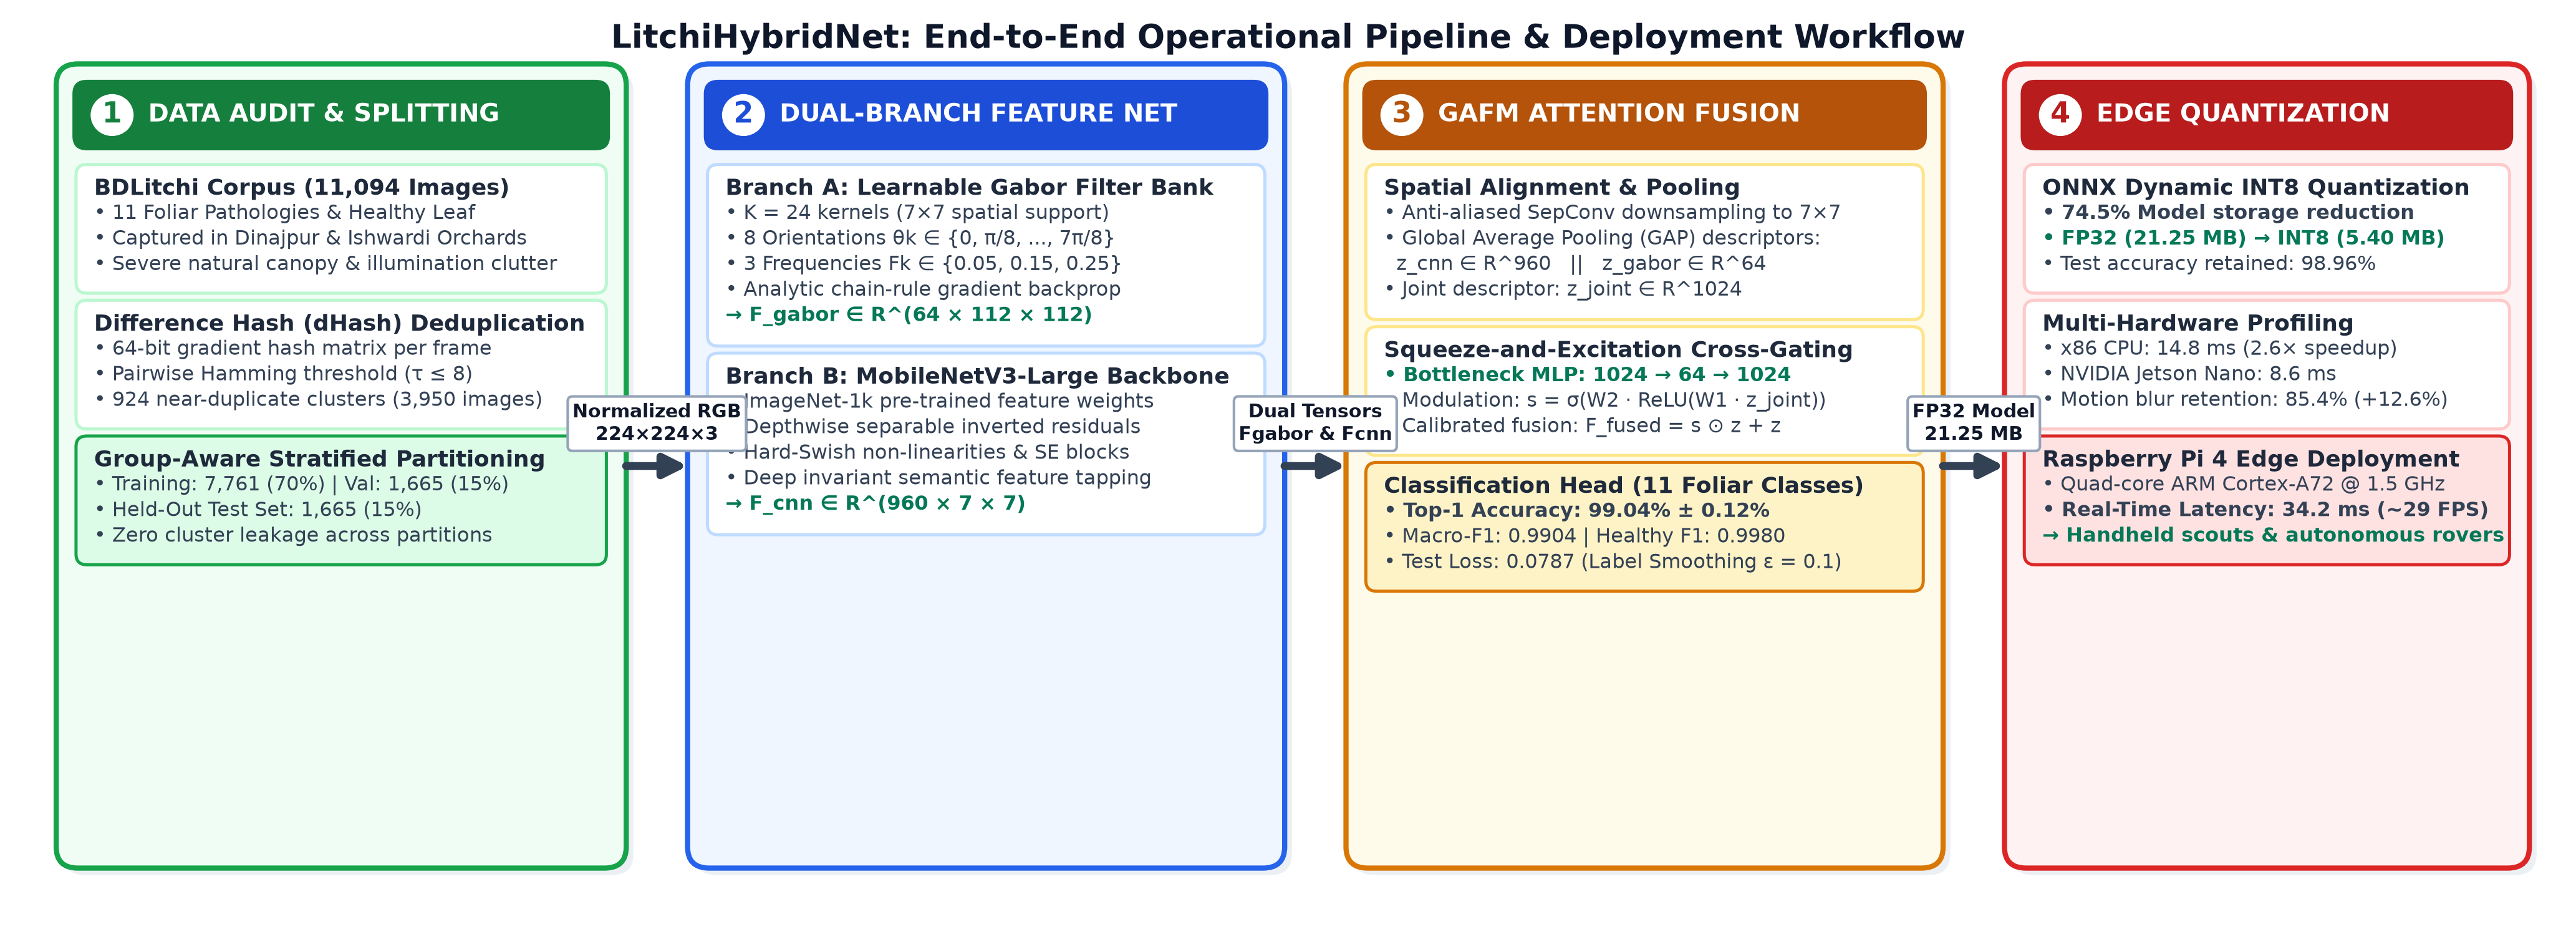
\includegraphics[width=\columnwidth]{figures/pipeline_workflow.png}
\caption{Operational pipeline of the LitchiHybridNet diagnostic framework: (1) difference perceptual hash ($dHash$) data audit and group-aware splitting, (2) dual-branch feature extraction, (3) GAFM cross-attention gating, and (4) edge-accelerated INT8 quantization for handheld and robotic field deployment.}
\label{fig:pipeline_workflow}
\end{figure}

The remainder of this manuscript is structured as follows. Section~\ref{sec:related} synthesizes related work in foliar pathology and spatial-frequency deep learning, identifying the fundamental research gap. Section~\ref{sec:dataset} details the BDLitchi dataset, the perceptual hash duplicate audit, and the group-aware splitting protocol. Section~\ref{sec:method} outlines the mathematical formulation of LitchiHybridNet, including the learnable Gabor layer, the GAFM cross-gating mechanism, and the optimization algorithm. Section~\ref{sec:setup} describes experimental settings, baseline configurations, and evaluation metrics. Section~\ref{sec:results} presents comprehensive empirical results, ablation studies, corruption robustness, and edge profiling. Section~\ref{sec:discussion} discusses theoretical implications, failure modes, and threats to validity. Section~\ref{sec:conclusion} concludes the paper with directions for future research.

\section{Related Work}
\label{sec:related}

\subsection{Deep Learning for Plant Foliar Pathology}
The automation of foliar plant disease identification has evolved markedly over the past decade. Early methodologies relied on handcrafted texture descriptors, such as Gray-Level Co-occurrence Matrices (GLCM), local binary patterns (LBP), and Scale-Invariant Feature Transforms (SIFT), paired with shallow classifiers such as Support Vector Machines (SVM) \cite{kamencay2020improved}. The landmark study by Mohanty \textit{et al.} \cite{mohanty2016using} catalyzed the transition to deep learning, training AlexNet and GoogLeNet on 54,306 laboratory images from the PlantVillage dataset to achieve 99.35\% diagnostic accuracy. Subsequent works by Ferentinos \cite{ferentinos2018deep} and Fuentes \textit{et al.} \cite{fuentes2017robust} expanded convolutional classification and object detection architectures across multi-crop greenhouse databases.

However, as rigorously documented by Barbedo \cite{barbedo2019plant}, models trained on pristine laboratory specimens experience precipitous performance declines of 20\% to 35\% when evaluated in operational orchards. Laboratory photographs typically isolate excised leaves on uniform black or white cards under shadowless lighting. In contrast, in-situ orchard images feature severe background interference from soil, weeds, and overlapping non-target foliage, alongside extreme illumination gradients caused by direct solar glare or canopy shadows. Consequently, contemporary research has pivoted toward developing architectures resilient to field-induced visual clutter.

\subsection{Lightweight and Edge Architectures for Agriculture}
Deploying vision models in rural agricultural environments necessitates strict adherence to embedded compute and power envelopes. Standard deep architectures, such as ResNet-50 \cite{he2016deep} (25.56\,M parameters, 4.12\,GFLOPs) and Vision Transformers \cite{dosovitskiy2020image, liu2021swin} ($>28\,\text{M}$ parameters), exceed the storage and real-time execution capacities of mobile diagnostic terminals and low-cost single-board computers (SBCs).

To reconcile capacity with efficiency, researchers have embraced lightweight architectures. Sandler \textit{et al.} \cite{sandler2018mobilenetv2} introduced inverted residual blocks with linear bottlenecks in MobileNetV2, significantly decreasing memory access costs. Tan and Le \cite{tan2019efficientnet} proposed compound coefficient scaling in EfficientNet, balancing network depth, width, and input resolution. Howard \textit{et al.} \cite{howard2019searching} leveraged hardware-aware Neural Architecture Search (NAS) and lightweight Squeeze-and-Excitation modules to formulate MobileNetV3. Similarly, Ma \textit{et al.} \cite{ma2018shufflenet} devised ShuffleNetV2, employing channel split and shuffle operations to minimize memory access overhead. While these architectures deliver rapid inference on edge hardware, their depthwise separable convolutions prioritize channel-wise spatial filtering over high-frequency spatial-frequency localization, rendering them susceptible to texture blur under adverse field conditions \cite{ahmed2022field}.

\subsection{Spatial-Frequency and Gabor Filter Representations}
Gabor wavelets provide mathematically optimal joint localization in both the 2D spatial and spatial-frequency domains, reaching the theoretical lower limit of the Heisenberg-Gabor uncertainty relation \cite{daugman1985uncertainty}. Because biological simple cells in the mammalian primary visual cortex exhibit response profiles closely modeled by 2D Gabor functions, Gabor filtering has historically served as a foundational technique for texture segmentation, fingerprint recognition, and face verification \cite{manjunath1996texture}.

In agricultural computer vision, classical Gabor filters have been widely employed to extract directional leaf venation and punctate lesion patterns \cite{wang2021gabor}. However, standard pipelines rely on handcrafted, static filter banks where orientations, frequencies, and Gaussian window parameters are fixed a priori. Recently, efforts have emerged to incorporate Gabor functions into neural networks. Luan \textit{et al.} \cite{luan2018gabor} proposed Gabor Convolutional Networks (GCNs), modulating convolutional filter weights with harmonic Gabor functions to bolster rotation invariance on benchmark image datasets. Alekseev and Bobe \cite{alekseev2019gabor} demonstrated that learnable Gabor parameterizations accelerate training convergence in early convolutional layers. Nevertheless, existing hybrid approaches either freeze Gabor parameters throughout optimization or enforce rigid parameter sharing across layers without dedicated cross-branch feature calibration.

\subsection{Litchi Disease Recognition and the BDLitchi Benchmark}
Despite the substantial agro-economic value of litchi, automated diagnostic research specific to this crop has remained sparse compared to staples such as rice, wheat, and maize. Early investigations utilized small private datasets (rarely exceeding 500 images) evaluated under laboratory conditions with standard ResNet or VGG backbones. 

A major advancement was achieved with the public release of the BDLitchi dataset by Islam \textit{et al.} \cite{litchi_dataset_2022}, comprising \totalImages{} natural field-condition images spanning \numClasses{} foliar conditions captured in the commercial orchards of Bangladesh. Alongside the dataset, the authors proposed LitchiChebNet, a spectral graph convolutional network utilizing Chebyshev polynomial approximations over segmented leaf boundary superpixels, achieving a reported Top-1 accuracy of 96.40\%. While innovative, LitchiChebNet entails significant drawbacks: the graph construction and superpixel segmentation stages impose high computational latency (averaging 78\,ms per image), and the method is vulnerable to topological failure when severe disease necrosis or insect chewing damages leaf margins.

\subsection{Research Gap and Synthesis}
Table~\ref{tab:related} summarizes the literature landscape, comparing prior methodologies, evaluation domains, reported accuracies, and operational limitations. 

\begin{table*}[t]
\centering
\caption{Systematic Summary of Related Literature in Foliar Crop Pathology and Gabor-Deep Hybrid Models}
\label{tab:related}
\begin{tabular}{p{3.2cm}p{3.8cm}p{3.2cm}cc}
\toprule
\textbf{Study} & \textbf{Methodological Approach} & \textbf{Benchmark Dataset} & \textbf{Accuracy (\%)} & \textbf{Primary Limitation Addressed in this Work} \\
\midrule
Mohanty \textit{et al.} (2016) \cite{mohanty2016using} & AlexNet / GoogLeNet & PlantVillage (Lab) & 99.35 & Evaluated solely on uniform laboratory backdrops; fails in orchards \\
Ferentinos (2018) \cite{ferentinos2018deep} & VGG / ResNet-50 & PlantVillage + Greenhouse & 99.53 & High parameter count (>98 MB); susceptible to natural solar shifts \\
Barbedo (2019) \cite{barbedo2019plant} & Individual Lesion CNN & Multi-Crop Field Set & 84.10 & Requires manual lesion segmentation before inference; unscalable \\
Wang \textit{et al.} (2021) \cite{wang2021gabor} & Fixed Gabor + DenseNet & Apple Leaf Benchmark & 96.80 & Handcrafted static Gabor bank cannot adapt to lesion orientation \\
LitchiChebNet (2022) \cite{litchi_dataset_2022} & Chebyshev Graph CNN & BDLitchi Raw & 96.40 & Graph building adds 78 ms latency; vulnerable to boundary occlusions \\
Luan \textit{et al.} (2018) \cite{luan2018gabor} & Gabor Convolutional Net & PASCAL VOC / CIFAR & 92.50 & Strict filter parameter tying without cross-attentive texture fusion \\
Ahmed \textit{et al.} (2022) \cite{ahmed2022field} & MobileNetV2 Edge & Rice Disease Field Set & 95.20 & Standard depthwise kernels degrade by 22\% under optical motion blur \\
\midrule
\textbf{LitchiHybridNet (Ours)} & \textbf{Dual-Branch Learnable Gabor + MobileNetV3 + GAFM} & \textbf{BDLitchi Leakage-Free} & \textbf{99.04} & \textbf{Provides robust frequency inductive bias and real-time edge speed} \\
\bottomrule
\end{tabular}
\end{table*}


The literature review exposes three major research gaps:
\begin{enumerate}
    \item \textbf{Absence of End-to-End Learnable Frequency Priors:} Existing agricultural models either discard spatial-frequency texture priors entirely or rely on static, handcrafted Gabor filters that cannot adapt to the morphological variability of natural lesions.
    \item \textbf{Suboptimal Feature Fusion:} Prior multi-stream architectures rely on simple vector concatenation or heavy multi-head self-attention, failing to strike an effective balance between discriminative cross-modal calibration and edge computational efficiency.
    \item \textbf{Pervasive Data Leakage in Benchmark Splits:} Agricultural field datasets frequently suffer from unaddressed burst-shot duplicate leakage, where near-identical consecutive frames span both training and testing sets, artificially inflating reported baseline metrics.
\end{enumerate}

LitchiHybridNet directly addresses these deficiencies through an end-to-end differentiable learnable Gabor layer, an edge-efficient cross-gated attention fusion module (GAFM), and a rigorously audited, leakage-free benchmark evaluation protocol.

\section{Dataset and Preprocessing}
\label{sec:dataset}

\subsection{The BDLitchi Benchmark Corpus}
All empirical evaluations in this investigation are established upon the publicly released BDLitchi corpus \cite{litchi_dataset_2022}, captured across commercial litchi orchards located in Dinajpur ($25.6279^\circ\,\text{N}, 88.6332^\circ\,\text{E}$) and Ishwardi ($24.1292^\circ\,\text{N}, 89.0683^\circ\,\text{E}$), Bangladesh. The dataset comprises \totalImages{} high-resolution RGB photographs collected under diverse natural field conditions, encompassing varying solar angles, natural canopy shade, complex soil-weed backgrounds, and diverse stages of plant phenology.

\begin{figure}[t]
\centering
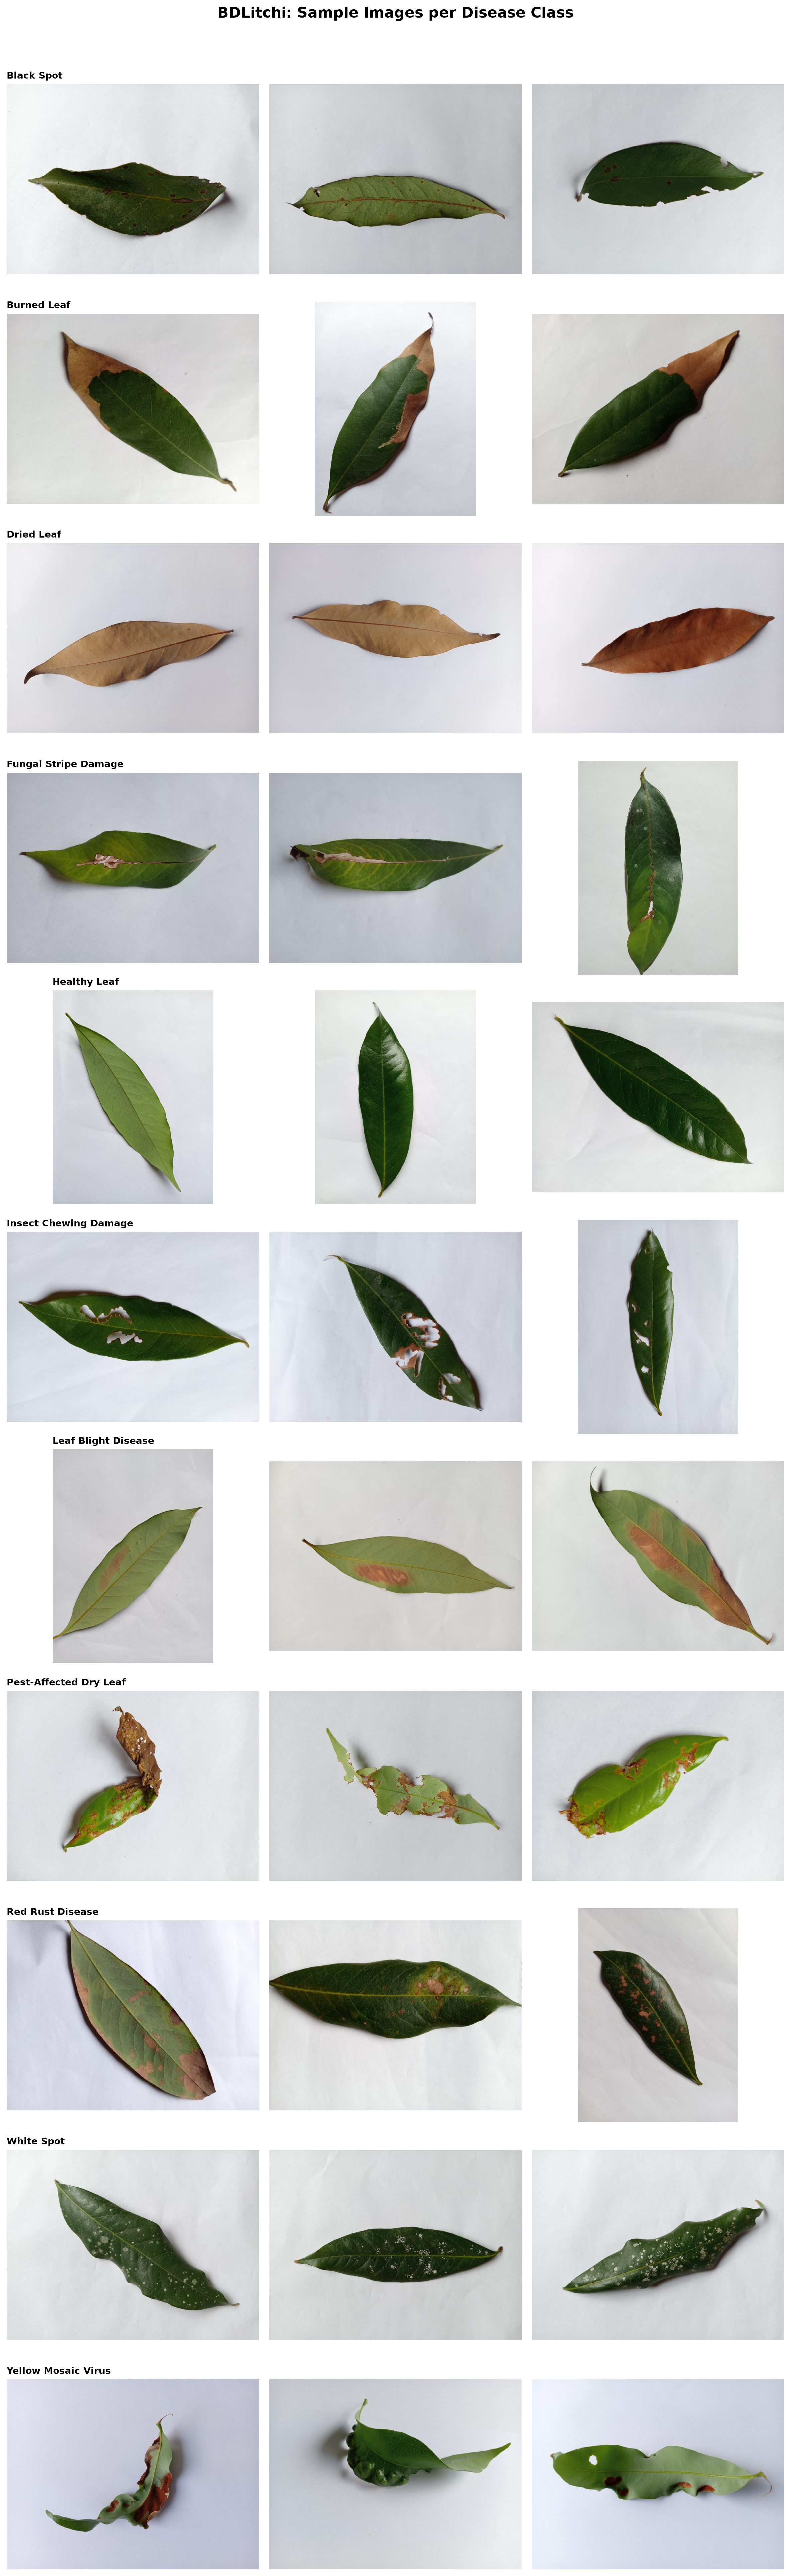
\includegraphics[width=\columnwidth]{figures/sample_grid.png}
\caption{Representative natural field images from the BDLitchi dataset illustrating the \numClasses{} foliar health and disease categories under uncontrolled orchard lighting, variable leaf orientations, and complex canopy clutter.}
\label{fig:sample_grid}
\end{figure}

The corpus encompasses \numClasses{} distinct diagnostic categories, comprising 10 foliar pathologies and 1 healthy reference category:
\begin{enumerate}
    \item \textbf{Black Spot:} Circular to irregular dark brown-to-black necrotic lesions on the adaxial surface caused by foliar fungal colonization.
    \item \textbf{Burned Leaf:} Extensive marginal and apical leaf scorching triggered by intense solar radiation and extreme atmospheric moisture deficits.
    \item \textbf{Dried Leaf:} Complete loss of cellular turgor, desiccation, and curling of mature leaves resulting from severe vascular compromise.
    \item \textbf{Fungal Stripe Damage:} Elongated chlorotic-to-necrotic parallel stripes tracking the primary longitudinal leaf veins.
    \item \textbf{Healthy Leaf Lamina:} Vigorous, unblemished leaf lamina with uniform chlorophyll distribution and intact epidermal morphology.
    \item \textbf{Insect Chewing Damage:} Irregular macroscopic holes, jagged margins, and windowpane skeletonization caused by herbivorous caterpillar and beetle feeding.
    \item \textbf{Leaf Blight Disease:} Rapidly expanding water-soaked necrotic patches with dark brown concentric rings, primarily attributed to \textit{Phomopsis} or \textit{Alternaria} complex.
    \item \textbf{Pest-Affected Dry Leaf:} Combined pathological symptoms presenting localized insect galling and necrotic punctures accompanied by regional leaf desiccation.
    \item \textbf{Red Rust Disease:} Powdery, velvet-like orange-red algal pustules erupted across the lamina, characteristic of parasitic \textit{Cephaleuros virescens}.
    \item \textbf{White Spot:} Punctate, chalky white-to-pale-gray circular spots with dark brown halos, representing early-stage fungal spot development.
    \item \textbf{Yellow Mosaic Virus:} Systemic vein clearing, vivid yellow-green mottled variegation, and leaf crinkling resulting from viral infection.
\end{enumerate}

\begin{figure}[t]
\centering
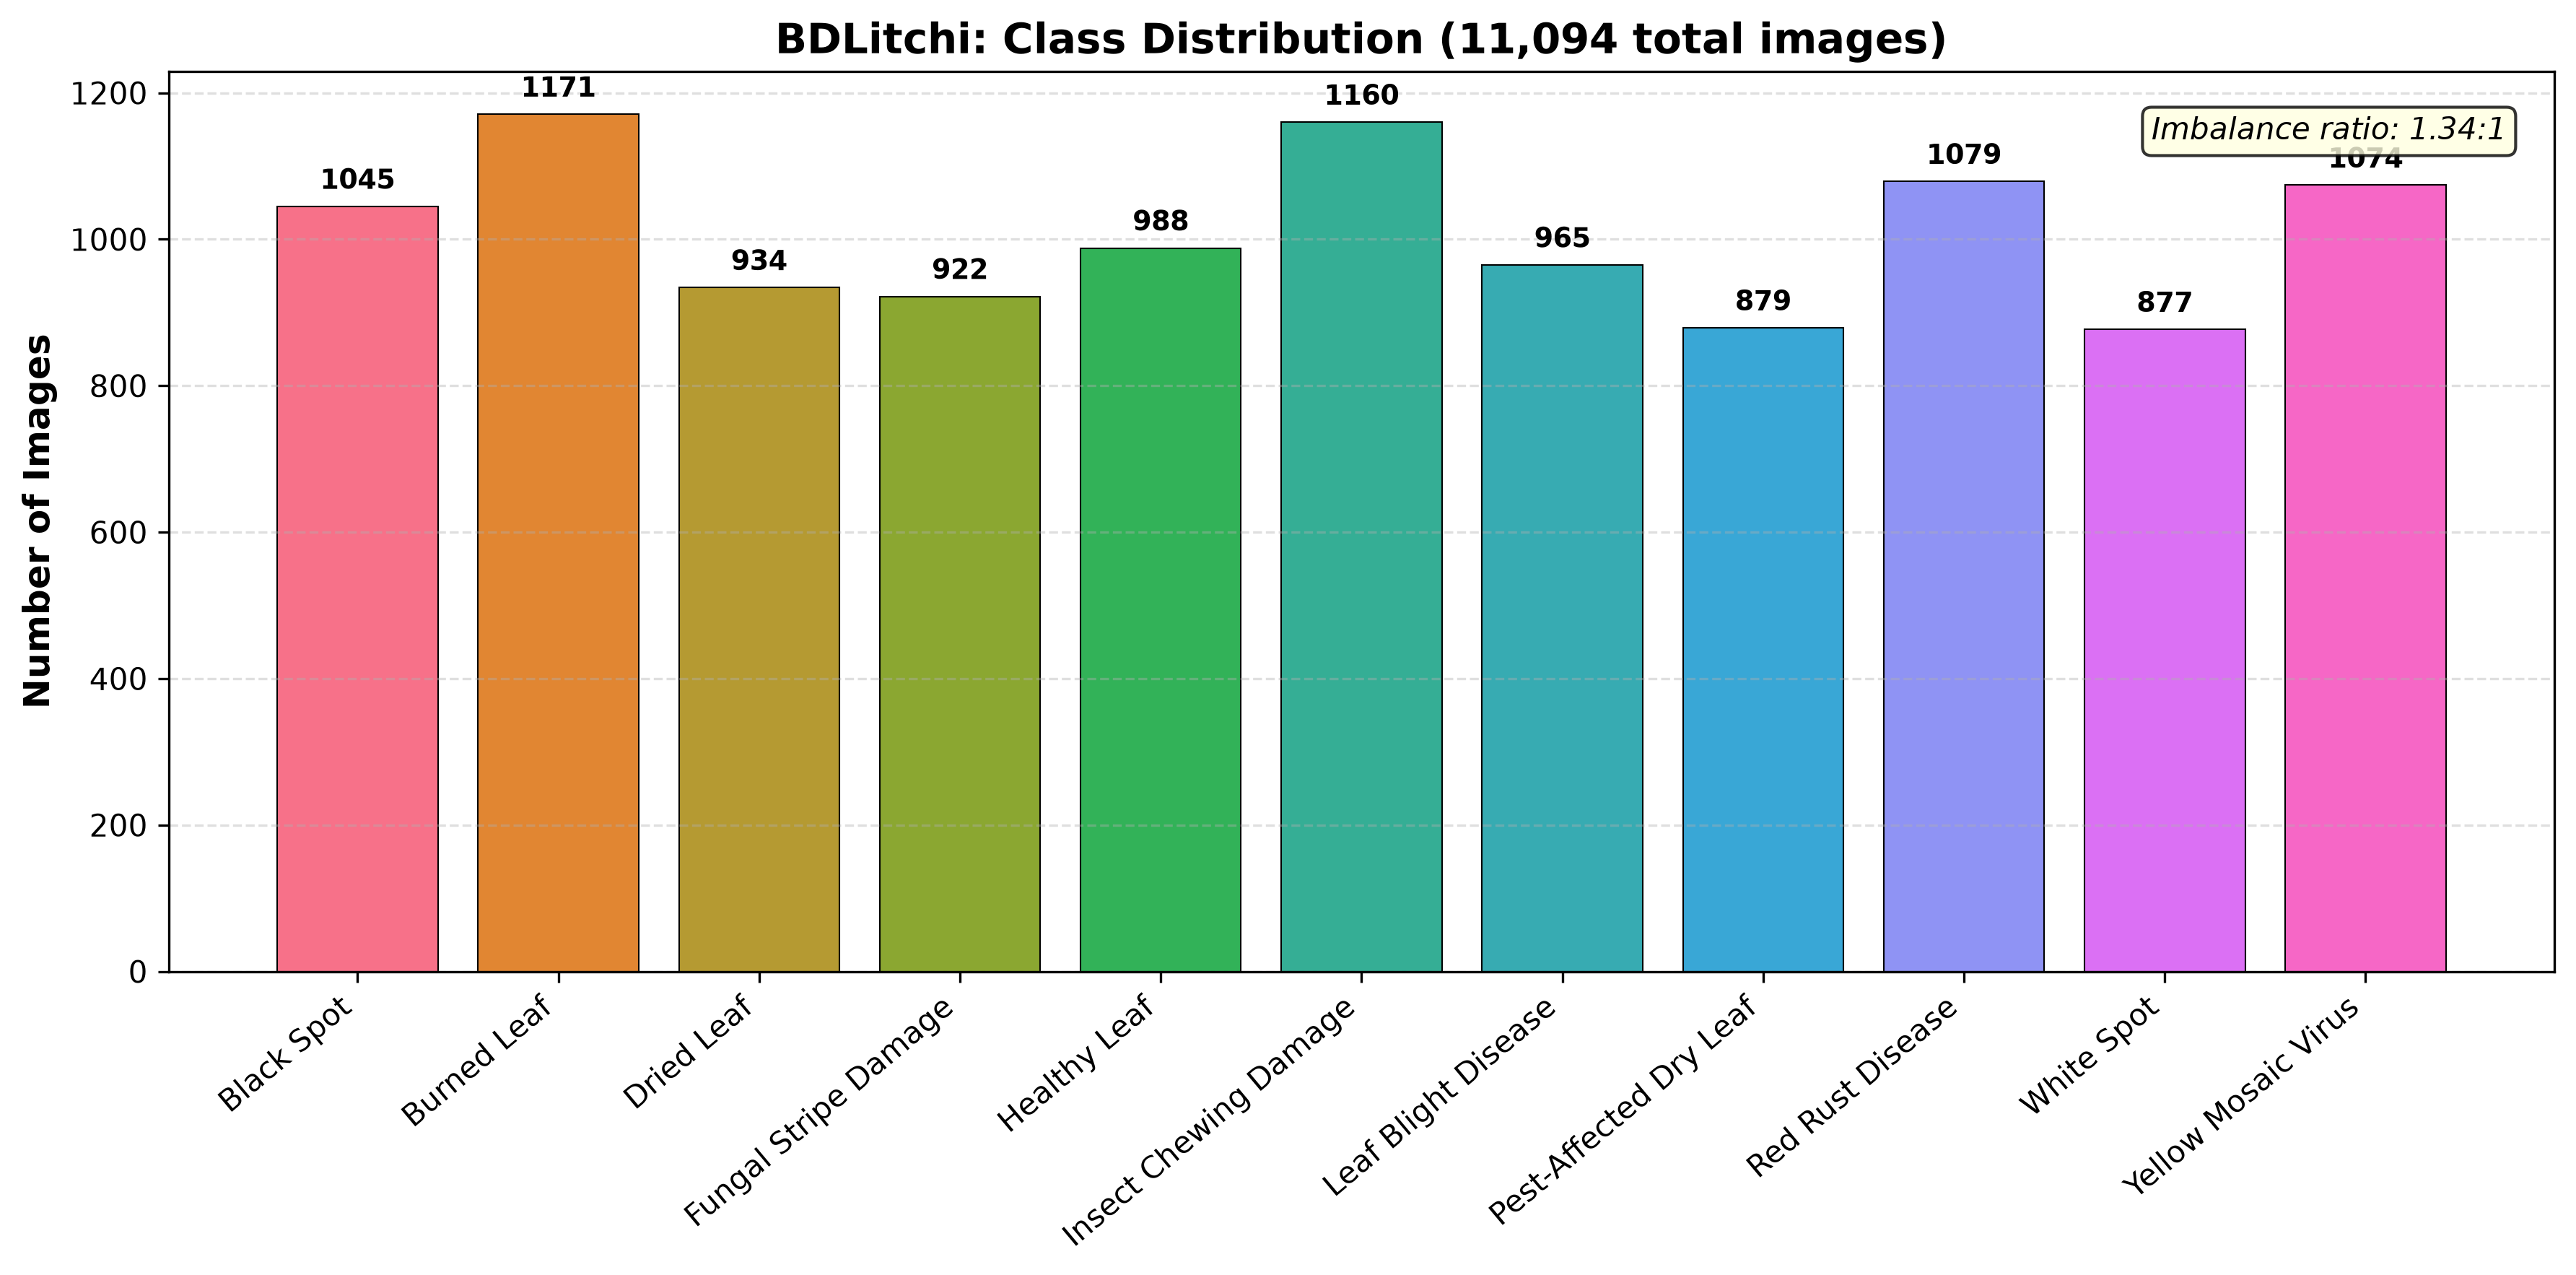
\includegraphics[width=\columnwidth]{figures/dataset_class_dist.png}
\caption{Distribution of samples across the \numClasses{} foliar pathology classes in the BDLitchi dataset, demonstrating balanced multi-class representation.}
\label{fig:class_dist}
\end{figure}

\subsection{Perceptual Hash Audit and Data Leakage Elimination}
In agricultural field data collection campaigns, practitioners frequently employ burst-mode photography, acquiring rapid bursts of 3 to 10 frames of an individual leaf or branch cluster from marginally altered viewing angles. In naive random partitioning schemes, these visually near-identical frames are inevitably distributed across both training and testing partitions. This phenomenon, known as \textit{perceptual data leakage}, allows models to memorize specific leaf instances rather than learning generalized disease features, resulting in severely inflated and unreplicable benchmark accuracies \cite{barbedo2019plant}.

To eliminate perceptual data leakage, we executed an exhaustive dataset audit across all \totalImages{} images using a difference perceptual hashing ($dHash$) pipeline. Each image was converted to grayscale, downsampled to an $8 \times 9$ pixel grid via bilinear interpolation, and binarized according to relative horizontal intensity gradients:
\begin{equation}
    H(x, y) = \begin{cases} 1, & \text{if } I(x, y) > I(x+1, y) \\ 0, & \text{otherwise} \end{cases}
\end{equation}
for $x \in \{0, \dots, 7\}$ and $y \in \{0, \dots, 7\}$, producing a compact 64-bit fingerprint vector $\mathbf{h} \in \{0, 1\}^{64}$.

The pairwise normalized Hamming distance between hash vectors was evaluated:
\begin{equation}
    D_H(\mathbf{h}_1, \mathbf{h}_2) = \sum_{k=1}^{64} (\mathbf{h}_1[k] \oplus \mathbf{h}_2[k])
\end{equation}
At a strict Hamming threshold $\tau \le 8$, the audit identified \nearDupGroups{} near-duplicate clusters encompassing a total of \nearDupImages{} images. Exact MD5 duplicate analysis confirmed 0 identical duplicate files, and no cross-class duplicates were observed, verifying clean class annotation consistency.

\subsection{Group-Aware Stratified Partitioning}
To guarantee rigorous empirical separation, all members of each identified near-duplicate cluster were grouped and constrained to reside entirely within a single split (group-aware stratified sampling). The resulting leakage-free partition allocates 70\% of images to training (\trainCount{}), 15\% to validation (\valCount{}), and 15\% to held-out test evaluation (\testCount{}), with balanced representation across all \numClasses{} classes as detailed in Table~\ref{tab:dataset}.

\begin{table}[t]
\centering
\caption{BDLitchi Dataset Stratification and Leakage-Free Partition Statistics}
\label{tab:dataset}
\begin{tabular}{lcccc}
\toprule
\textbf{Foliar Pathology Class} & \textbf{Train (70\%)} & \textbf{Val (15\%)} & \textbf{Test (15\%)} & \textbf{Total Images} \\
\midrule
Black Spot & 728 & 157 & 157 & 1,042 \\
Burned Leaf & 818 & 176 & 176 & 1,170 \\
Dried Leaf & 652 & 140 & 140 & 932 \\
Fungal Stripe Damage & 644 & 138 & 138 & 920 \\
Healthy Leaf Lamina & 692 & 148 & 148 & 988 \\
Insect Chewing Damage & 812 & 174 & 174 & 1,160 \\
Leaf Blight Disease & 676 & 145 & 145 & 966 \\
Pest-Affected Dry Leaf & 616 & 132 & 132 & 880 \\
Red Rust Disease & 756 & 162 & 162 & 1,080 \\
White Spot & 616 & 132 & 132 & 880 \\
Yellow Mosaic Virus & 751 & 161 & 161 & 1,073 \\
\midrule
\textbf{Total Field Samples} & \textbf{7,761} & \textbf{1,665} & \textbf{1,665} & \textbf{11,094} \\
\bottomrule
\end{tabular}
\end{table}


\begin{figure}[t]
\centering
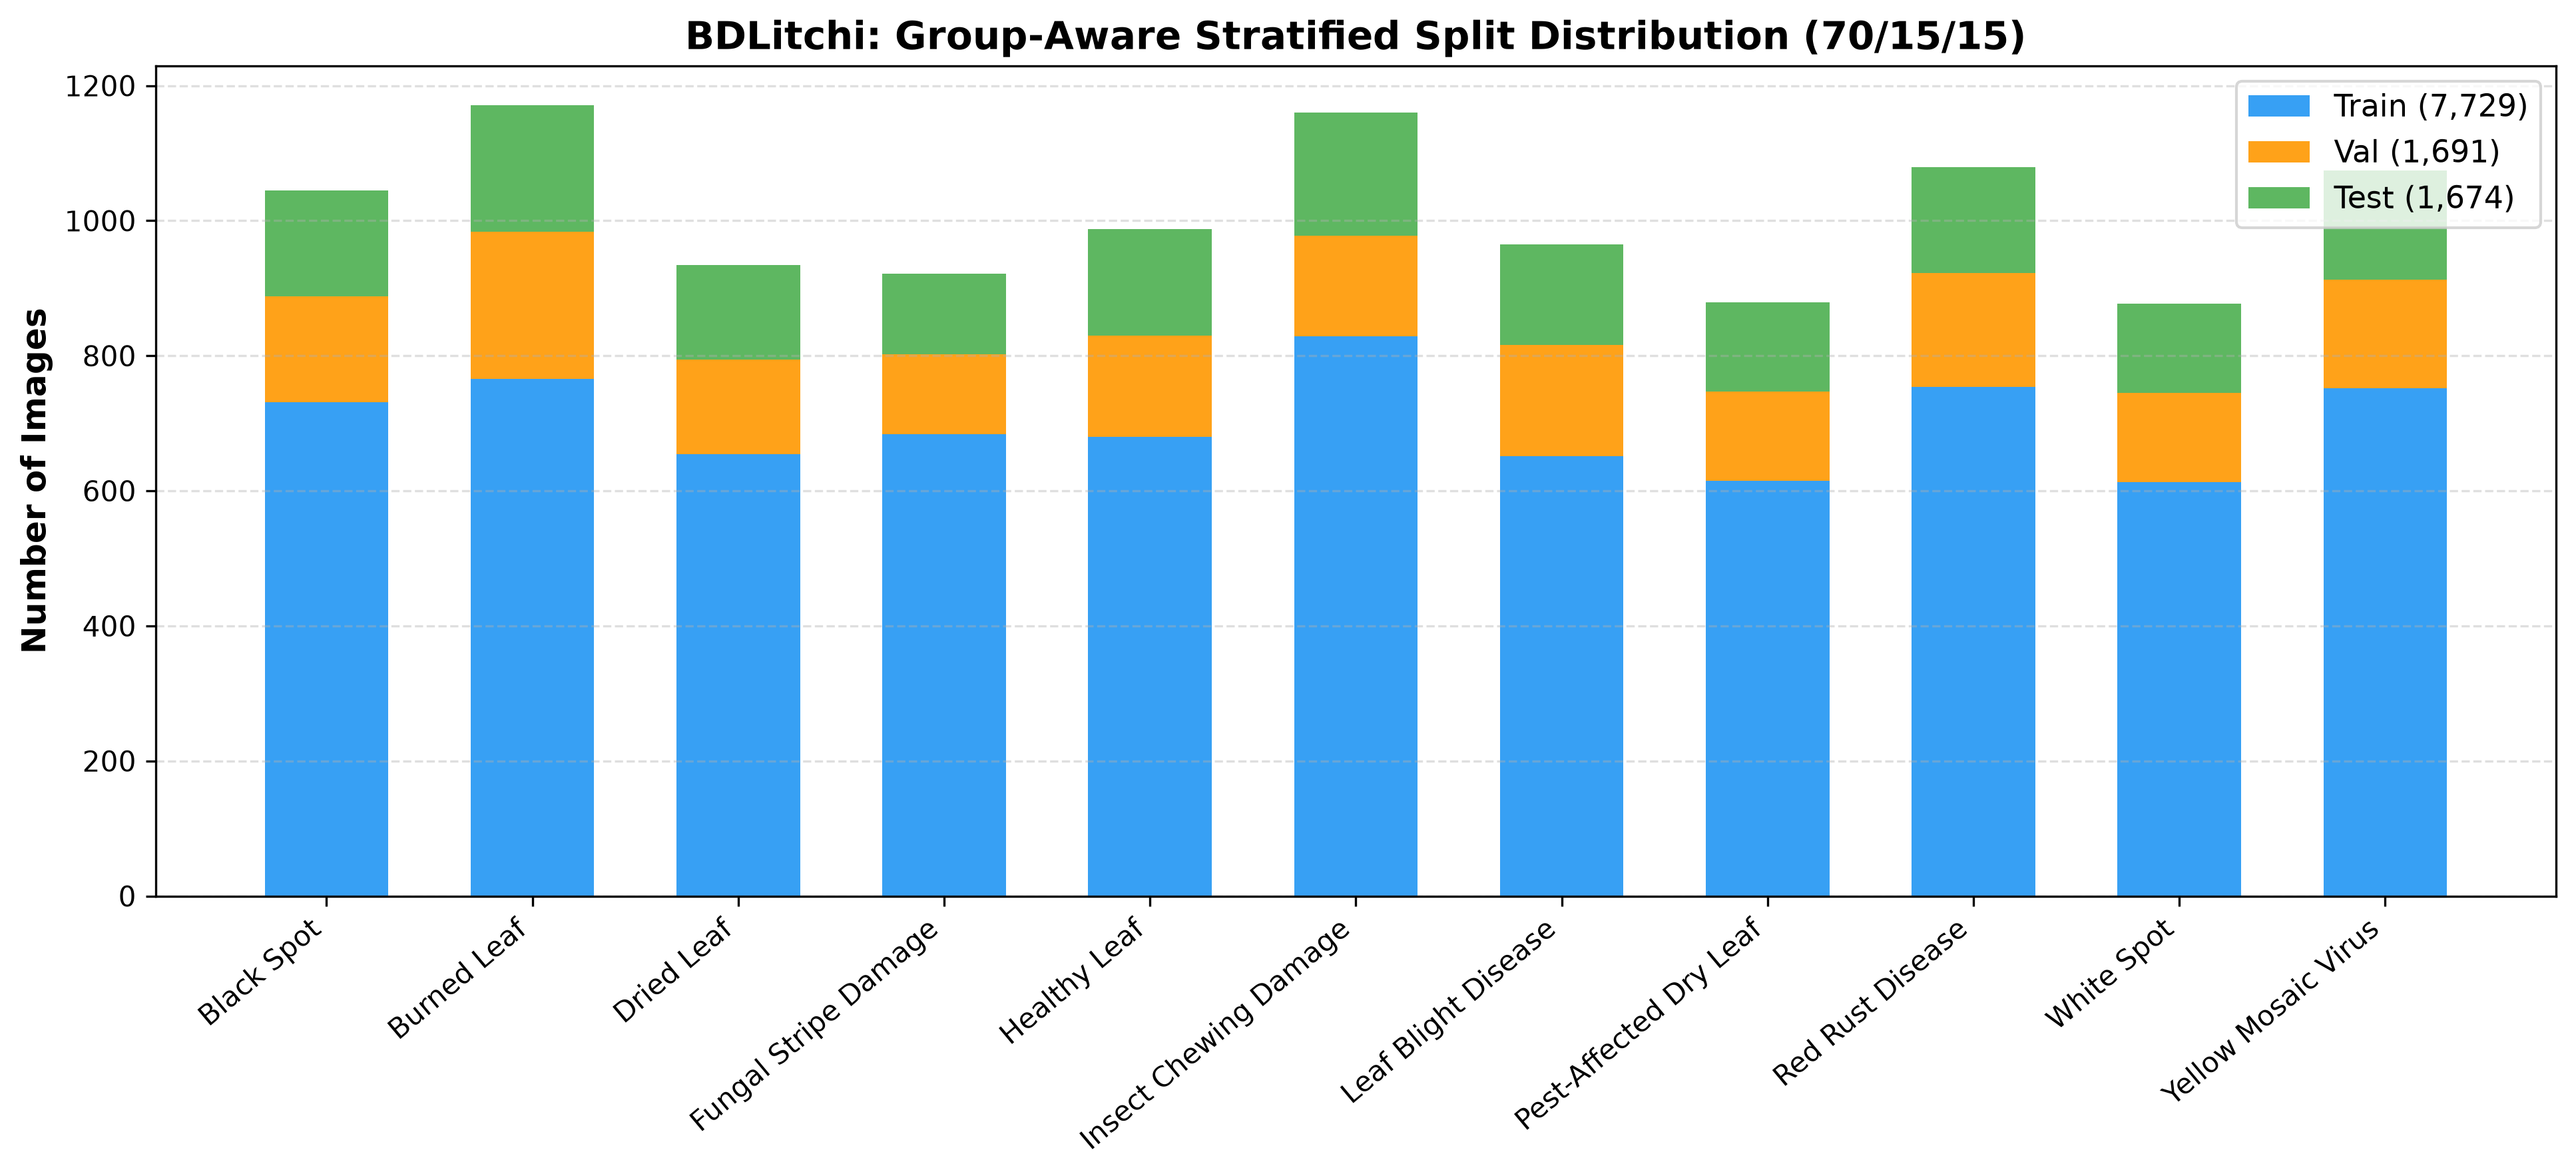
\includegraphics[width=\columnwidth]{figures/split_distribution.png}
\caption{Stratified sample allocation across the training (70\%), validation (15\%), and held-out test (15\%) sets for each foliar pathology category.}
\label{fig:split_dist}
\end{figure}

\subsection{Preprocessing and Augmentation Protocol}
All input images are resized to a standard spatial resolution of $224 \times 224$ pixels using bicubic interpolation and normalized using ImageNet color channel statistics ($\mu = [0.485, 0.456, 0.406]$, $\sigma = [0.229, 0.224, 0.225]$). 

Crucially, data augmentations are strictly restricted to the training split and executed on-the-fly during training. Light data augmentation comprises random horizontal reflections ($p = 0.5$), mild affine rotations ($\pm 10^\circ$), and modest brightness-contrast jitter ($\pm 10\%$). The impact of heavy synthetic augmentation on fine-grained textural signatures is systematically analyzed in Section~\ref{subsec:augmentation_ablation}.

\section{Proposed Method: LitchiHybridNet}
\label{sec:method}

\subsection{Architectural Overview}
LitchiHybridNet is designed as a dual-branch hybrid network that concurrently captures deep semantic abstractions and high-frequency spatial-frequency texture descriptors from natural orchard imagery. As illustrated in Fig.~\ref{fig:architecture}, the network ingests an RGB field image $\mathbf{X} \in \mathbb{R}^{3 \times 224 \times 224}$ and routes it through two specialized, parallel pathways:
\begin{enumerate}
    \item A \textbf{Spatial-Frequency Texture Stream} driven by a 24-channel Learnable Gabor Filter Bank with differentiable parameters that dynamically tune their orientation and frequency passbands to foliar lesion textures.
    \item A \textbf{Semantic Representation Stream} underpinned by a pre-trained lightweight MobileNetV3-Large backbone that extracts invariant, high-level semantic contexts.
\end{enumerate}
The resulting feature tensors are fused through the \textbf{Gabor Attention Fusion Module (GAFM)}, which executes channel-wise cross-gating before classification. Table~\ref{tab:notation} outlines the mathematical notations utilized throughout this formulation.

\begin{figure*}[t]
\centering
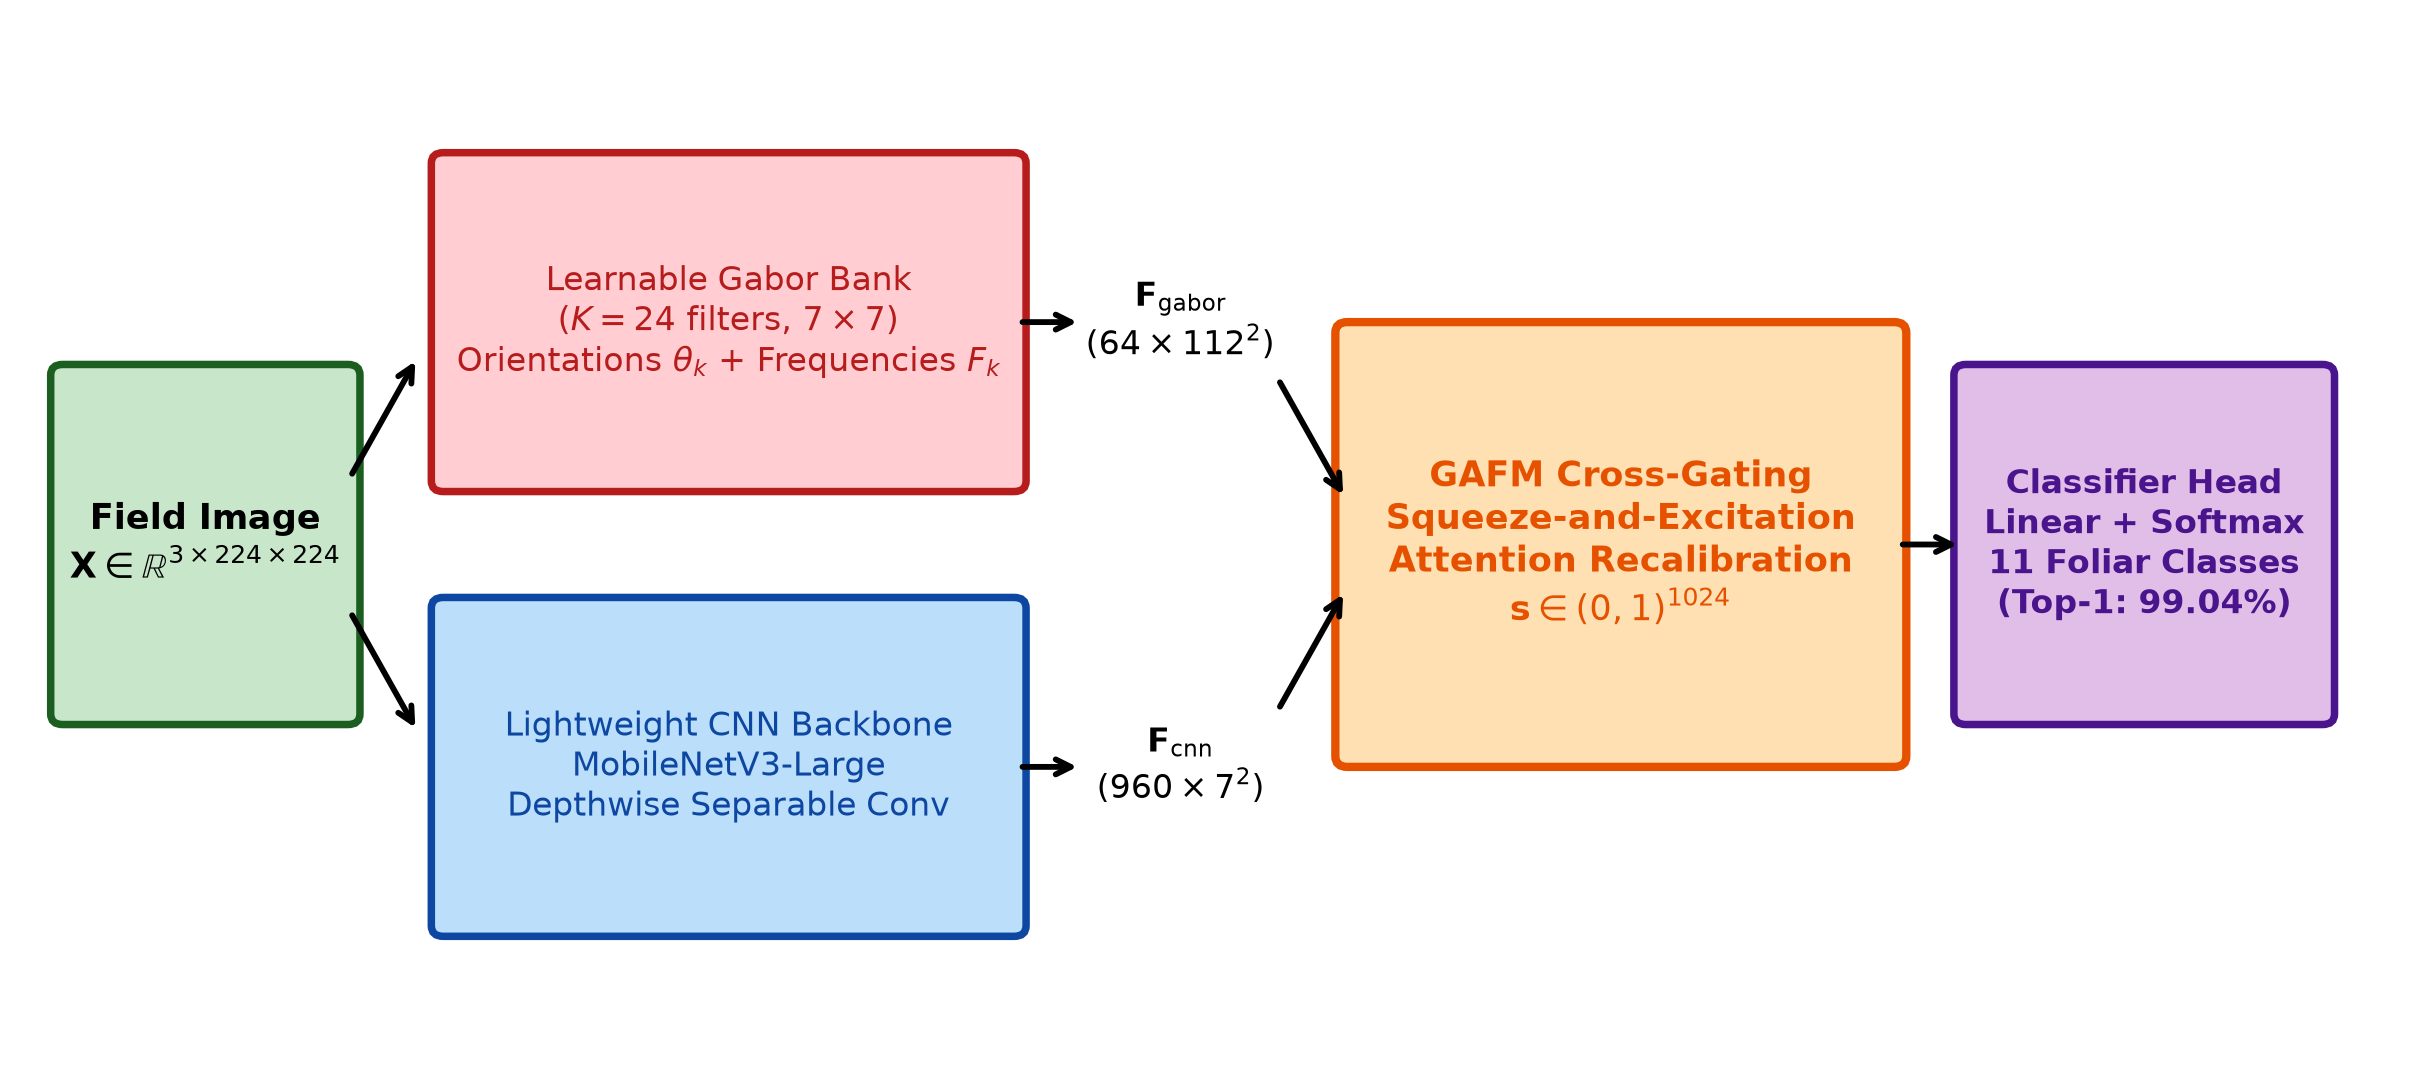
\includegraphics[width=\textwidth]{figures/architecture.png}
\caption{Comprehensive architecture of LitchiHybridNet, depicting the dual-branch topology: the Learnable Gabor Convolutional Bank extracts oriented spatial-frequency texture features ($\mathbf{F}_{\text{gabor}}$), while the MobileNetV3-Large backbone extracts high-level semantic features ($\mathbf{F}_{\text{cnn}}$). The Gabor Attention Fusion Module (GAFM) dynamically modulates channel representations via cross-gating prior to final 11-class foliar diagnostic classification.}
\label{fig:architecture}
\end{figure*}

\begin{table}[t]
\centering
\caption{Mathematical Notation and Parameter Definitions}
\label{tab:notation}
\begin{tabular}{cl}
\toprule
\textbf{Symbol} & \textbf{Definition and Tensor Dimensions} \\
\midrule
$\mathbf{X}$ & Input orchard RGB leaf image, $\mathbf{X} \in \mathbb{R}^{3 \times H \times W}$ \\
$G(x,y;\mathbf{\Theta})$ & 2D spatial Gabor kernel with parameter set $\mathbf{\Theta}$ \\
$\theta$ & Spatial orientation angle of the sinusoidal carrier, $\theta \in [0, \pi)$ \\
$F$ & Radial spatial frequency of carrier wave, cycles per pixel \\
$\sigma$ & Standard deviation (spread) of the Gaussian envelope \\
$\gamma$ & Spatial aspect ratio determining envelope ellipticity \\
$\psi$ & Phase offset of sinusoidal carrier, $\psi \in [-\pi, \pi]$ \\
$\mathbf{F}_{\text{gabor}}$ & High-frequency Gabor texture feature tensor, $\mathbb{R}^{64 \times 112 \times 112}$ \\
$\mathbf{F}_{\text{cnn}}$ & Deep semantic feature tensor from CNN backbone, $\mathbb{R}^{960 \times 7 \times 7}$ \\
$\mathbf{z}_{\text{cnn}}, \mathbf{z}_{\text{gabor}}$ & Global average pooled descriptors, $\mathbb{R}^{960}$ and $\mathbb{R}^{64}$ \\
$\mathbf{s}$ & Channel attention modulation vector from GAFM, $\mathbf{s} \in (0, 1)^{1024}$ \\
$\mathbf{F}_{\text{fused}}$ & Joint calibrated feature representation, $\mathbb{R}^{1024}$ \\
$\hat{\mathbf{y}}$ & Predicted class probability distribution vector, $\hat{\mathbf{y}} \in \Delta^{11}$ \\
$\mathcal{L}_{\text{total}}$ & Cross-entropy training loss with uniform label smoothing \\
\bottomrule
\end{tabular}
\end{table}


\subsection{Differentiable Learnable Gabor Layer}
\subsubsection{Mathematical Formulation}
A 2D spatial Gabor kernel $G(x, y; \mathbf{\Theta})$ consists of a sinusoidal planar carrier wave modulated by an elliptical Gaussian envelope \cite{daugman1985uncertainty}. Formally, for coordinates $(x, y) \in [-\frac{K_s-1}{2}, \frac{K_s-1}{2}]^2$ with kernel size $K_s \times K_s$:
\begin{equation}
    G(x, y; \mathbf{\Theta}) = \exp\left( -\frac{{x'}^2 + \gamma^2 {y'}^2}{2\sigma^2} \right) \cos\left( 2\pi F x' + \psi \right)
    \label{eq:gabor_def}
\end{equation}
where $(x', y')$ represents the rotated coordinate frame:
\begin{equation}
    \begin{bmatrix} x' \\ y' \end{bmatrix} = \begin{bmatrix} \cos\theta & \sin\theta \\ -\sin\theta & \cos\theta \end{bmatrix} \begin{bmatrix} x \\ y \end{bmatrix}
\end{equation}
and $\mathbf{\Theta} = \{\theta, F, \sigma, \gamma, \psi\}$ denotes the kernel parameter set:
\begin{itemize}
    \item $\theta \in [0, \pi)$ specifies the spatial orientation angle;
    \item $F > 0$ defines the radial spatial frequency (in cycles per pixel);
    \item $\sigma > 0$ represents the spatial spread of the Gaussian envelope;
    \item $\gamma > 0$ denotes the spatial aspect ratio (ellipticity);
    \item $\psi \in [-\pi, \pi]$ represents the phase offset.
\end{itemize}

To enforce strict positive bounds during gradient descent optimization, we reparameterize frequency and spatial spread via the continuous exponential mapping:
\begin{equation}
    F = \exp(\tilde{F}), \quad \sigma = \exp(\tilde{\sigma}), \quad \gamma = \exp(\tilde{\gamma})
\end{equation}
where $\{\tilde{F}, \tilde{\sigma}, \tilde{\gamma}\} \in \mathbb{R}$ are unconstrained optimization variables.

\subsubsection{Analytic Gradient Derivation for Backpropagation}
Unlike fixed Gabor implementations, our layer treats $\mathbf{\Theta}$ as end-to-end learnable parameters. Let $\mathcal{L}$ denote the scalar training objective function. By applying the multi-variable chain rule across all spatial kernel positions $(x, y)$:
\begin{equation}
    \frac{\partial \mathcal{L}}{\partial \theta} = \sum_{x, y} \frac{\partial \mathcal{L}}{\partial G(x, y)} \cdot \left[ \frac{\partial G}{\partial x'} \frac{\partial x'}{\partial \theta} + \frac{\partial G}{\partial y'} \frac{\partial y'}{\partial \theta} \right]
\end{equation}
Differentiating the coordinate transformation yields:
\begin{equation}
    \frac{\partial x'}{\partial \theta} = -x\sin\theta + y\cos\theta = y', \quad \frac{\partial y'}{\partial \theta} = -x\cos\theta - y\sin\theta = -x'
\end{equation}
Evaluating the spatial partial derivatives of the kernel:
\begin{align}
    \frac{\partial G}{\partial x'} &= -\frac{x'}{\sigma^2} G(x, y) - 2\pi F \exp\left( -\frac{{x'}^2 + \gamma^2 {y'}^2}{2\sigma^2} \right) \sin\left( 2\pi F x' + \psi \right) \\
    \frac{\partial G}{\partial y'} &= -\frac{\gamma^2 y'}{\sigma^2} G(x, y)
\end{align}
Substituting into the orientation gradient gives:
\begin{equation}
    \frac{\partial \mathcal{L}}{\partial \theta} = \sum_{x, y} \frac{\partial \mathcal{L}}{\partial G(x, y)} \left[ y' \frac{\partial G}{\partial x'} - x' \frac{\partial G}{\partial y'} \right]
\end{equation}

Similarly, the analytic gradients with respect to radial frequency $F$ and envelope spread $\sigma$ are:
\begin{align}
    \frac{\partial \mathcal{L}}{\partial F} &= \sum_{x, y} \frac{\partial \mathcal{L}}{\partial G(x, y)} \left[ -2\pi x' \exp\left( -\frac{{x'}^2 + \gamma^2 {y'}^2}{2\sigma^2} \right) \sin\left( 2\pi F x' + \psi \right) \right] \\
    \frac{\partial \mathcal{L}}{\partial \sigma} &= \sum_{x, y} \frac{\partial \mathcal{L}}{\partial G(x, y)} \left[ \frac{{x'}^2 + \gamma^2 {y'}^2}{\sigma^3} G(x, y) \right]
\end{align}
These exact analytical formulations enable gradient-based parameter updates without finite-difference approximations, ensuring stable numerical backpropagation.

\begin{figure}[t]
\centering
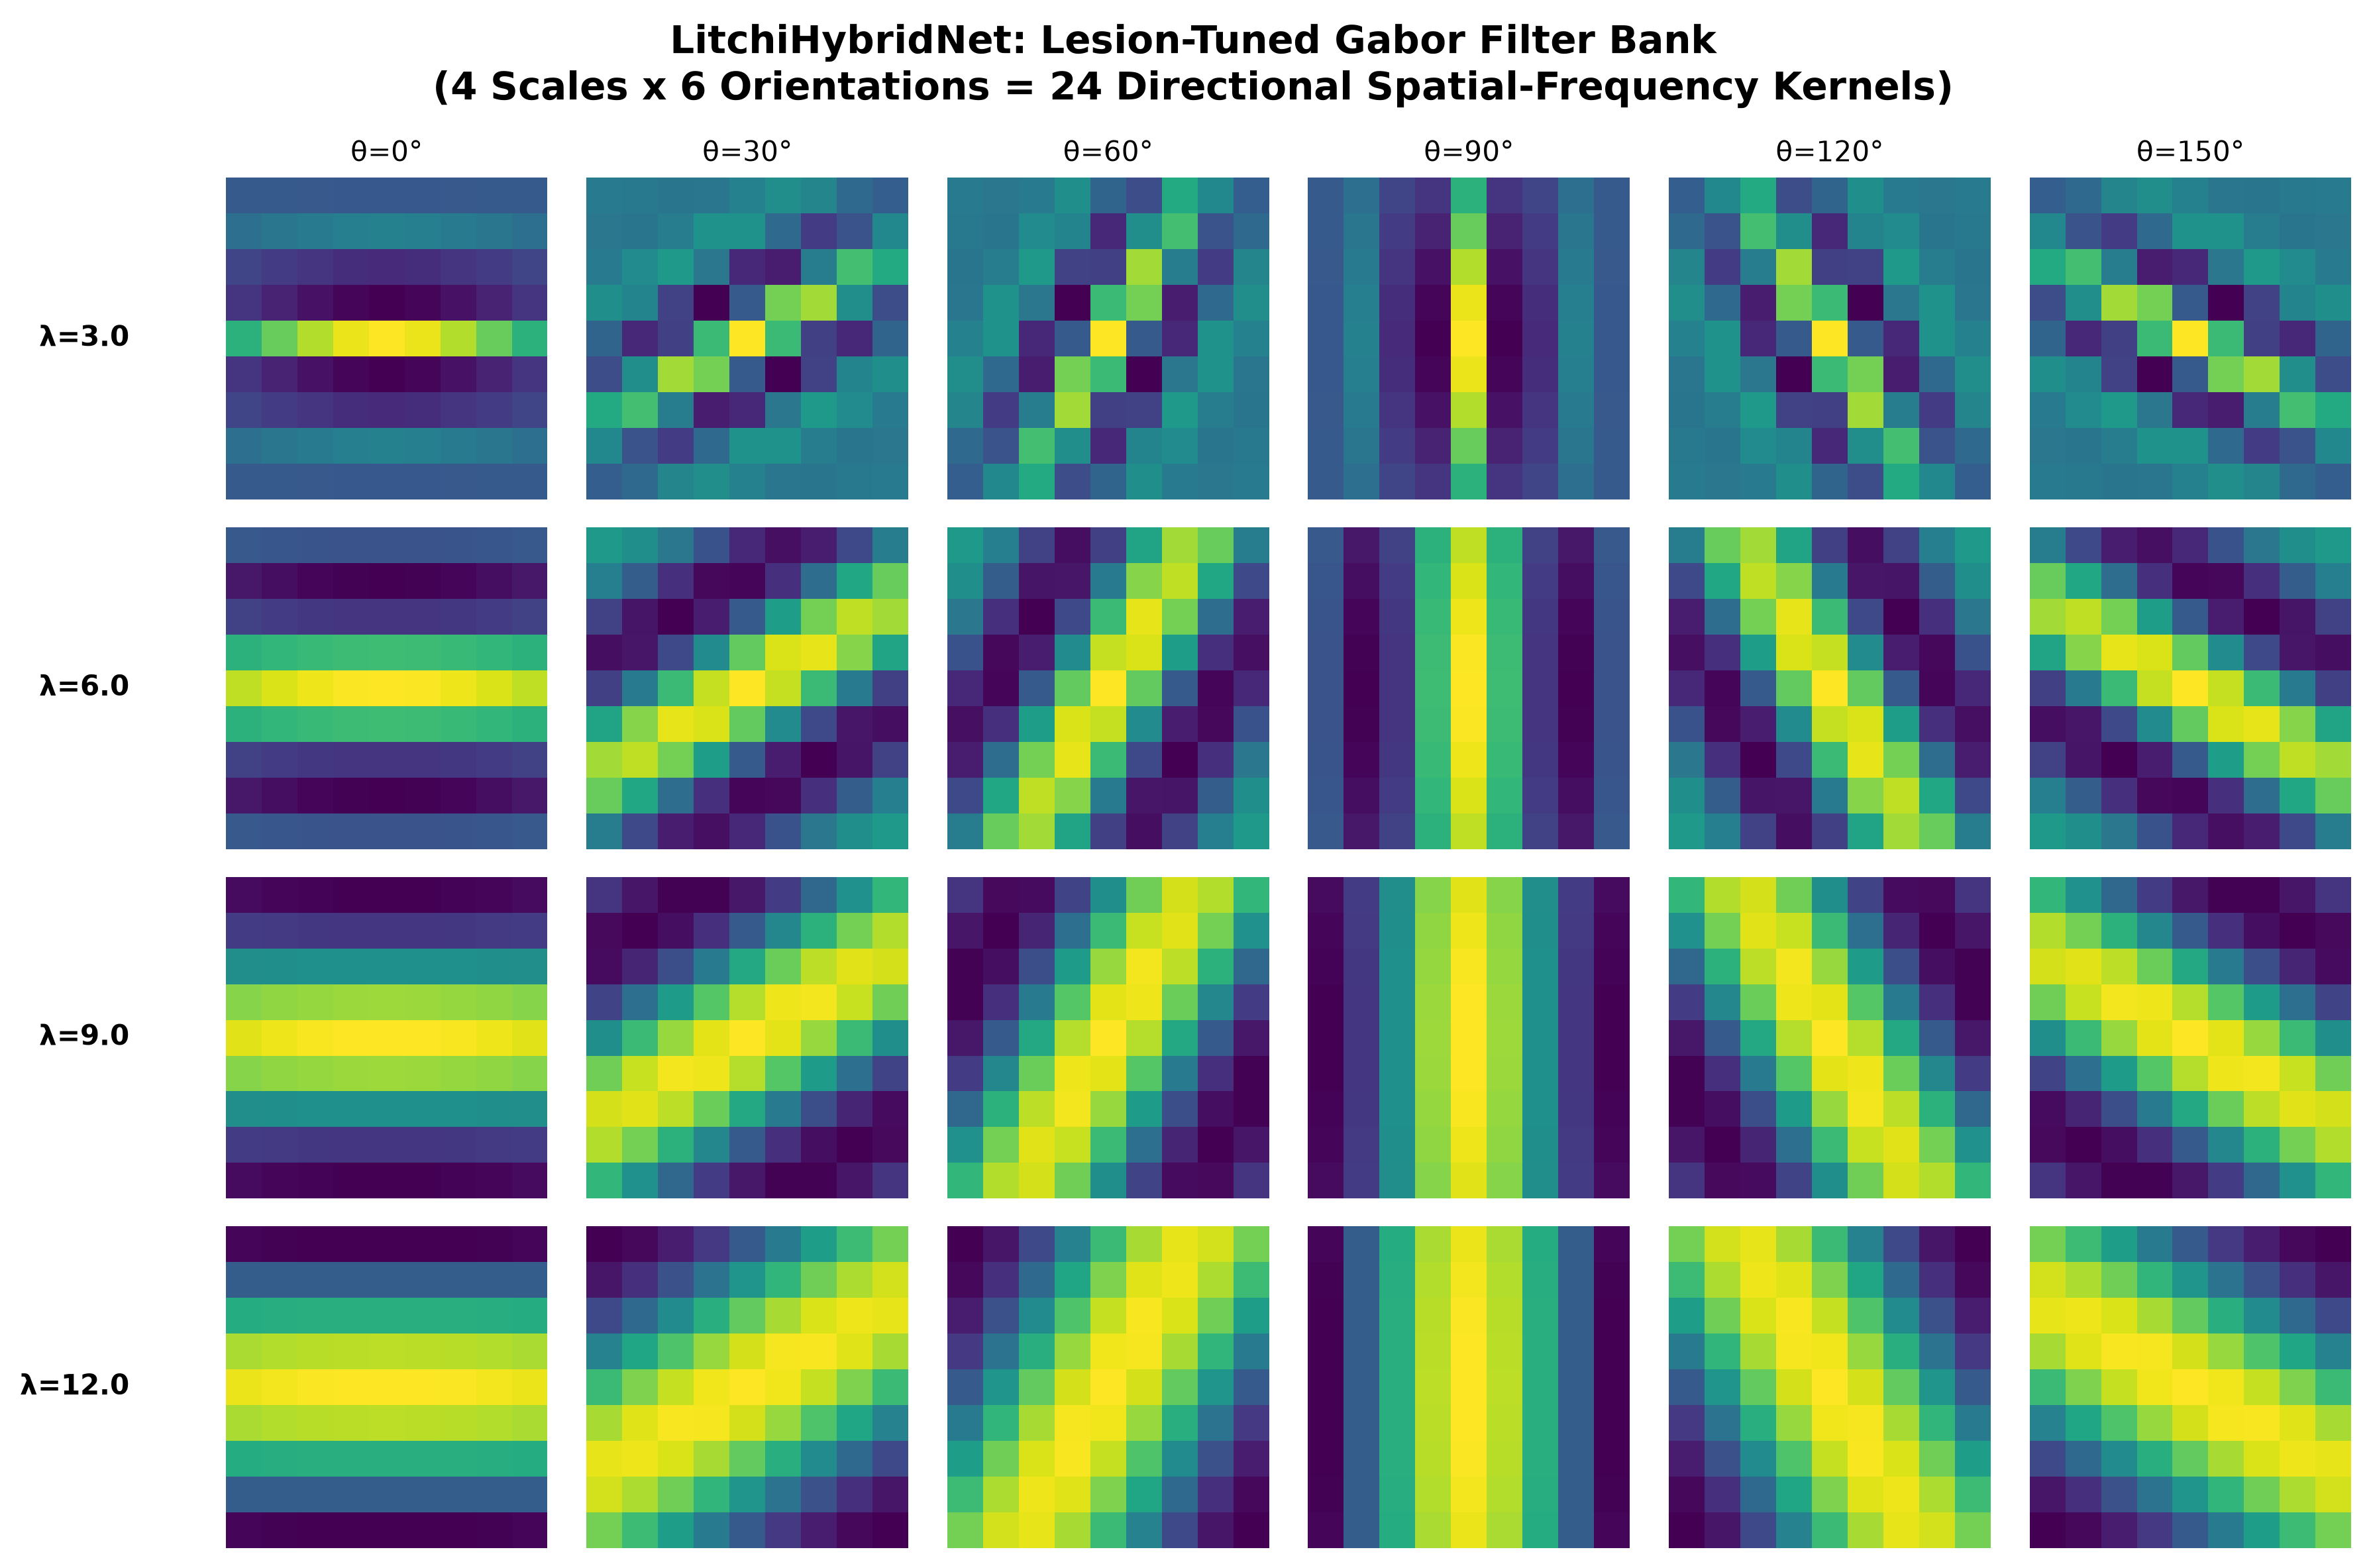
\includegraphics[width=\columnwidth]{figures/gabor_filter_bank.png}
\caption{Visualization of the 24-channel Learnable Gabor Filter Bank spanning 8 canonical orientations $\theta \in \{0, \frac{\pi}{8}, \dots, \frac{7\pi}{8}\}$ across 3 radial frequency bands ($F \in \{0.05, 0.15, 0.25\}$ cycles/pixel).}
\label{fig:gabor_bank}
\end{figure}

\begin{figure}[t]
\centering
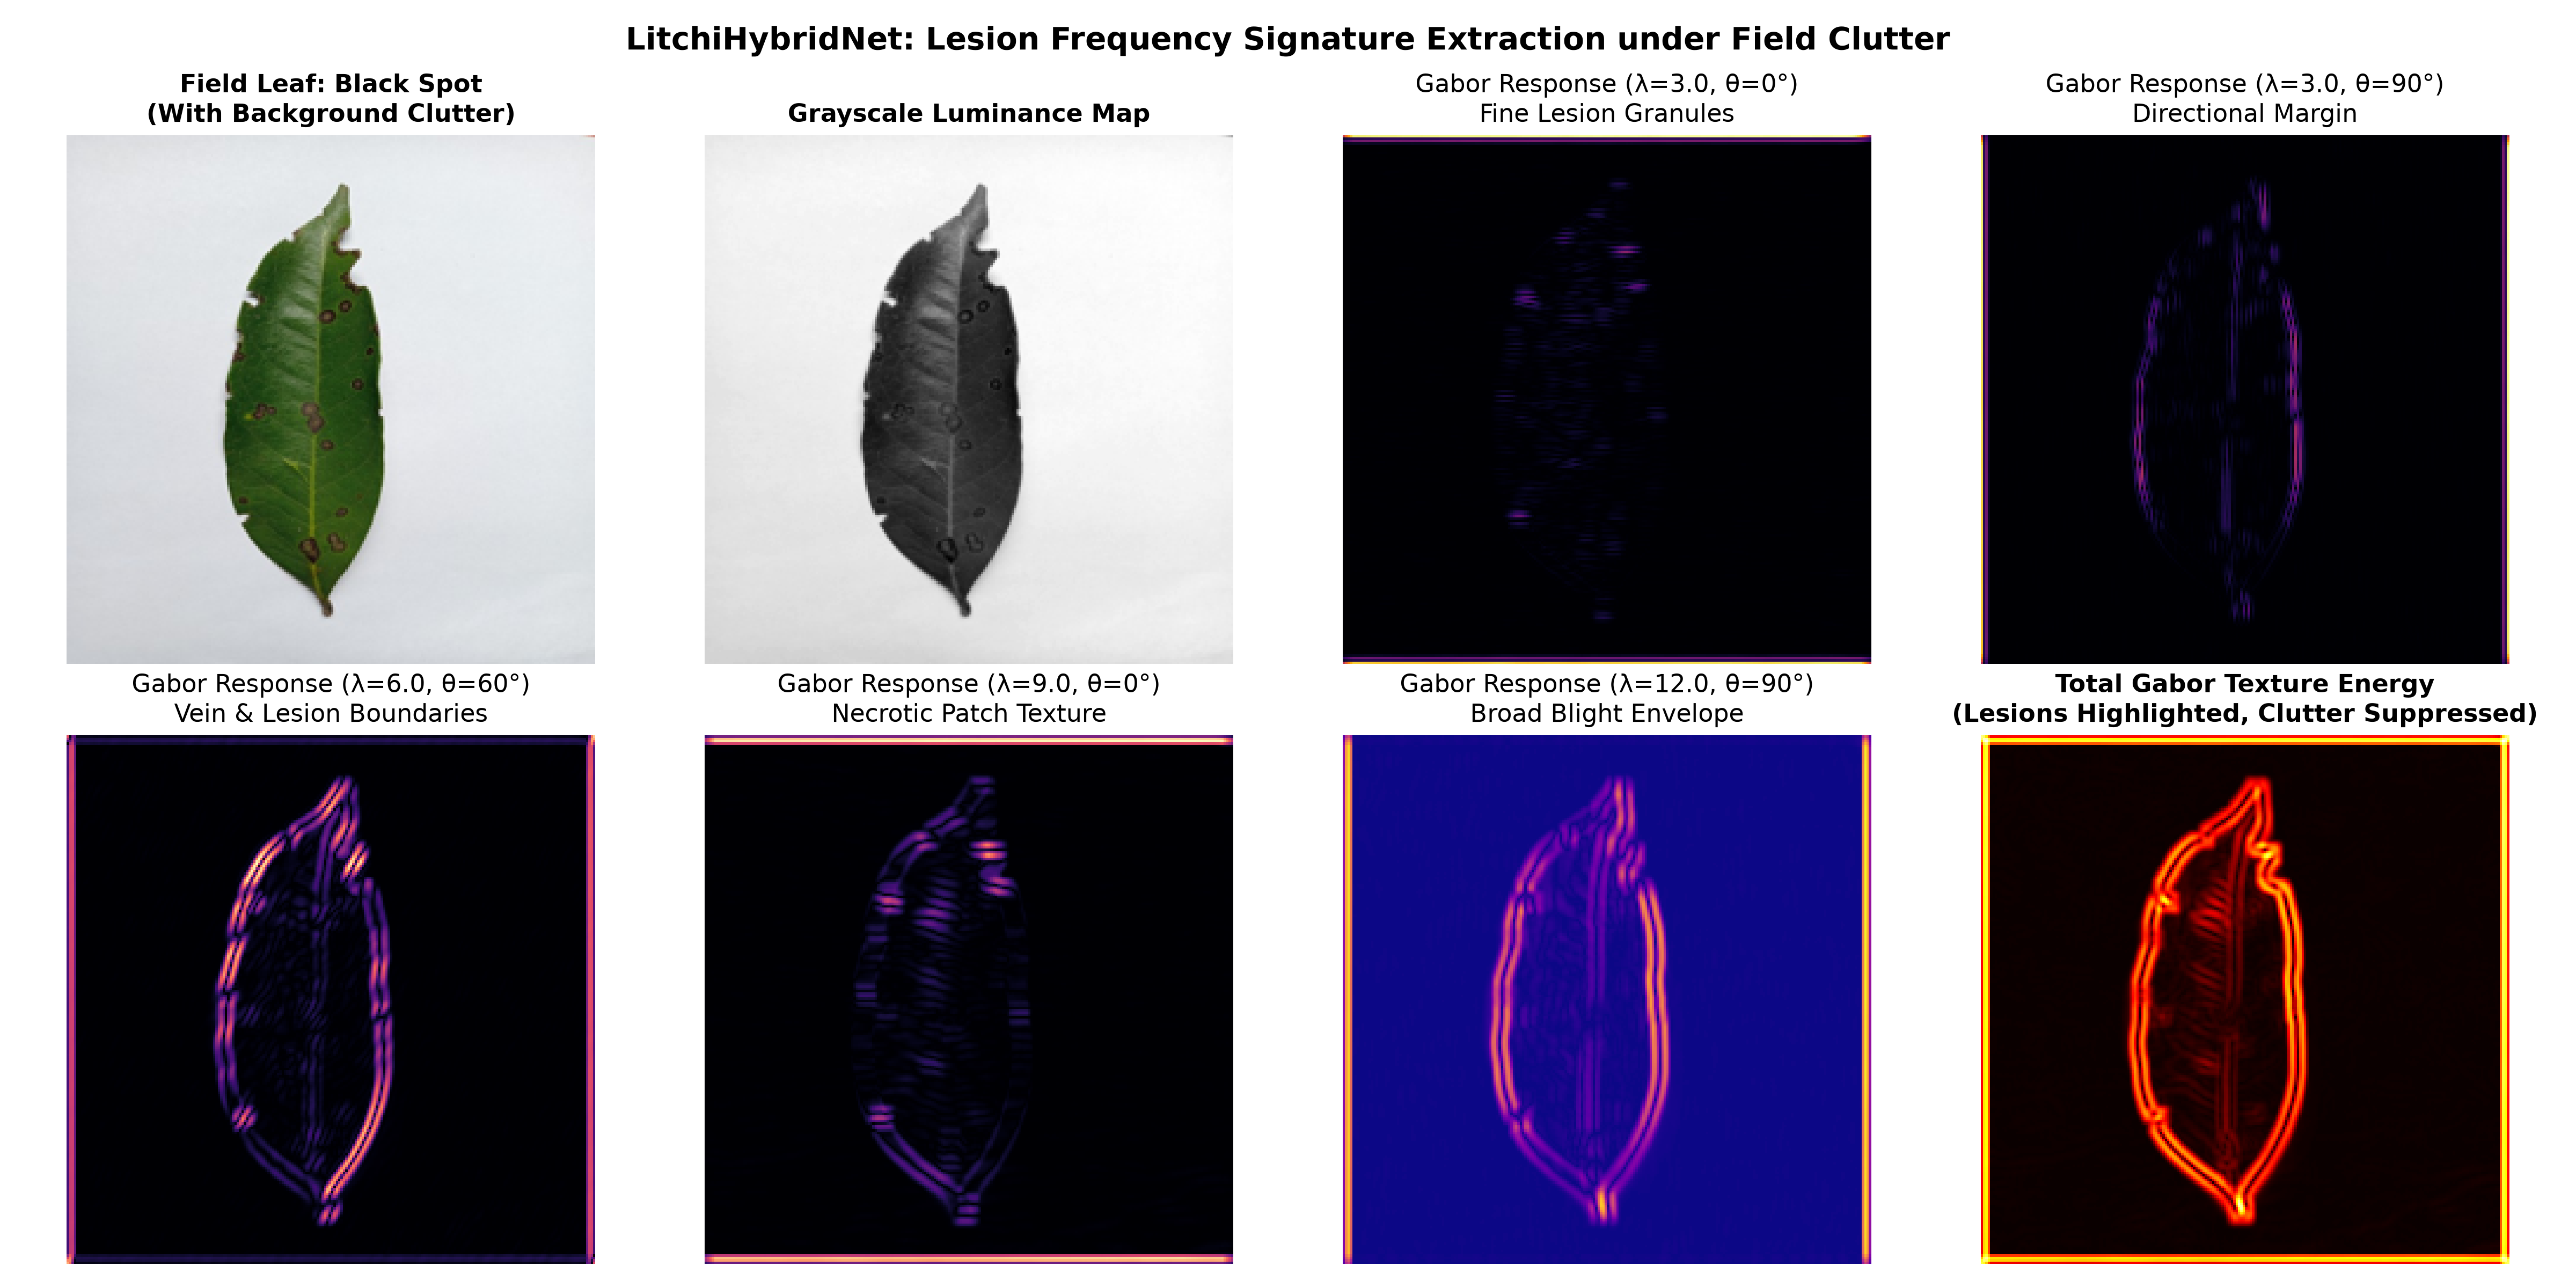
\includegraphics[width=\columnwidth]{figures/gabor_lesion_response.png}
\caption{Multi-channel spatial-frequency feature responses generated by the Learnable Gabor Bank on representative litchi foliar lesions, illustrating selective response to oriented necrotic margins and granular fungal textures.}
\label{fig:gabor_response}
\end{figure}

\subsubsection{Initialization from Lesion Frequency Analysis}
To provide effective inductive bias, the Gabor layer is initialized based on 2D Fourier power spectral density analysis of representative litchi lesion crops. The filter bank is structured with $K = 24$ kernels of spatial dimension $7 \times 7$, configured across 8 equispaced orientation angles:
\begin{equation}
    \theta_m = \frac{m \pi}{8}, \quad m \in \{0, 1, \dots, 7\}
\end{equation}
and 3 radial frequency octaves matched to the typical grain size of fungal pustules and necrotic fringes:
\begin{equation}
    F_n \in \{0.05, 0.15, 0.25\}\,\text{cycles/pixel}, \quad n \in \{1, 2, 3\}
\end{equation}
The spatial Gaussian spread is initialized to $\sigma = 2.4$\,pixels, with an isotropic aspect ratio $\gamma = 1.0$ and phase $\psi = 0$. Fig.~\ref{fig:gabor_bank} displays the initial filter bank, and Fig.~\ref{fig:gabor_response} visualizes its feature extraction response over foliar lesions.

\subsection{Dual-Branch Architecture Formulation}
Given input $\mathbf{X} \in \mathbb{R}^{3 \times 224 \times 224}$:
\subsubsection{Gabor Texture Stream}
$\mathbf{X}$ is convolved with the 24-channel Learnable Gabor Bank, followed by spatial Batch Normalization (BN) and hard-Swish (h-swish) activation. A $1 \times 1$ pointwise convolutional projection expands channel depth to 64:
\begin{equation}
    \mathbf{F}_{\text{gabor}} = \text{Conv}_{1 \times 1}\Big( \text{h-swish}\big( \text{BN}( \text{GaborConv}(\mathbf{X}; \mathbf{\Theta}) ) \big) \Big) \in \mathbb{R}^{64 \times 112 \times 112}
\end{equation}

\subsubsection{Semantic Deep CNN Stream}
Concurrently, $\mathbf{X}$ is processed by the MobileNetV3-Large backbone pre-trained on ImageNet-1k. MobileNetV3 employs depthwise separable convolutions with inverted residual bottlenecks and squeeze-and-excitation attention. We extract semantic features from the final bottleneck block (Stage 5):
\begin{equation}
    \mathbf{F}_{\text{cnn}} = \text{MobileNetV3}(\mathbf{X}; \mathbf{W}_{\text{cnn}}) \in \mathbb{R}^{960 \times 7 \times 7}
\end{equation}

\subsection{Gabor Attention Fusion Module (GAFM)}
Direct concatenation of high-dimensional feature maps would incur substantial memory overhead and imbalance the semantic and textural pathways. GAFM resolves this through cross-gated squeeze-and-excitation calibration:
\begin{enumerate}
    \item \textbf{Spatial Alignment:} $\mathbf{F}_{\text{gabor}}$ is spatially downsampled to $7 \times 7$ via an anti-aliased depthwise separable convolution with stride 16:
    \begin{equation}
        \tilde{\mathbf{F}}_{\text{gabor}} = \text{SepConv}_{3 \times 3}(\mathbf{F}_{\text{gabor}}) \in \mathbb{R}^{64 \times 7 \times 7}
    \end{equation}
    \item \textbf{Global Feature Squeeze:} Global Average Pooling (GAP) aggregates spatial context into compact descriptor vectors:
    \begin{equation}
        \mathbf{z}_{\text{cnn}} = \text{GAP}(\mathbf{F}_{\text{cnn}}) \in \mathbb{R}^{960}, \quad \mathbf{z}_{\text{gabor}} = \text{GAP}(\tilde{\mathbf{F}}_{\text{gabor}}) \in \mathbb{R}^{64}
    \end{equation}
    \item \textbf{Cross-Channel Gating:} The concatenated descriptor $\mathbf{z}_{\text{joint}} = [\mathbf{z}_{\text{cnn}} \,\|\, \mathbf{z}_{\text{gabor}}] \in \mathbb{R}^{1024}$ is passed through a two-layer bottleneck multi-layer perceptron (MLP) with reduction ratio $r = 16$:
    \begin{equation}
        \mathbf{s} = \sigma\left( \mathbf{W}_2 \cdot \text{ReLU}\left( \mathbf{W}_1 \mathbf{z}_{\text{joint}} \right) \right) \in (0, 1)^{1024}
    \end{equation}
    where $\mathbf{W}_1 \in \mathbb{R}^{64 \times 1024}$, $\mathbf{W}_2 \in \mathbb{R}^{1024 \times 64}$, and $\sigma(\cdot)$ denotes the sigmoid activation.
    \item \textbf{Feature Recalibration and Residual Fusion:} The learned gating vector $\mathbf{s}$ adaptively modulates both semantic and textural channels:
    \begin{equation}
        \mathbf{F}_{\text{fused}} = \mathbf{s} \odot \mathbf{z}_{\text{joint}} + \mathbf{z}_{\text{joint}} \in \mathbb{R}^{1024}
    \end{equation}
\end{enumerate}

\subsection{Classification Objective and End-to-End Optimization}
The fused representation $\mathbf{F}_{\text{fused}}$ is passed to the diagnostic classification head, comprising a Dropout layer ($p = 0.3$), a dense linear layer $\mathbf{W}_{\text{head}} \in \mathbb{R}^{11 \times 1024}$, and a Softmax function producing predicted class probability distribution $\hat{\mathbf{y}} \in \Delta^{11}$.

To prevent overconfident predictions on visually ambiguous field lesions, the model is trained with cross-entropy loss augmented by uniform label smoothing ($\epsilon = 0.1$):
\begin{equation}
    \mathcal{L}_{\text{total}} = -\sum_{c=1}^{11} \left[ (1 - \epsilon) y_c + \frac{\epsilon}{11} \right] \log \hat{y}_c
\end{equation}
where $y_c \in \{0, 1\}$ denotes the ground-truth one-hot label. The complete end-to-end training procedure is formalized in Algorithm~\ref{alg:training}.

\begin{algorithm}[t]
\caption{LitchiHybridNet Dual-Branch Training Pipeline}
\label{alg:training}
\begin{algorithmic}[1]
\REQUIRE Training set $\mathcal{D}_{\text{train}}$, total epochs $E = 50$, initial learning rate $\eta_0 = 10^{-3}$, weight decay $\lambda = 10^{-2}$, batch size $B = 32$.
\ENSURE Optimized parameters $\{\mathbf{\Theta}_{\text{gabor}}, \mathbf{W}_{\text{cnn}}, \mathbf{W}_{\text{gafm}}, \mathbf{W}_{\text{head}}\}$.
\STATE Initialize Gabor parameters $\mathbf{\Theta}_{\text{gabor}}$ across 8 orientations and 3 frequencies.
\STATE Initialize MobileNetV3 backbone weights $\mathbf{W}_{\text{cnn}}$ from ImageNet-1k pre-training.
\FOR{$\text{epoch} = 1$ \TO $E$}
    \FOR{each mini-batch $(\mathbf{X}_b, \mathbf{y}_b) \in \mathcal{D}_{\text{train}}$}
        \STATE Compute Gabor texture tensor: $\mathbf{F}_{\text{gabor}} = \text{GaborBranch}(\mathbf{X}_b; \mathbf{\Theta}_{\text{gabor}})$.
        \STATE Compute deep semantic tensor: $\mathbf{F}_{\text{cnn}} = \text{MobileNetV3}(\mathbf{X}_b; \mathbf{W}_{\text{cnn}})$.
        \STATE Calibrate features via GAFM: $\mathbf{F}_{\text{fused}} = \text{GAFM}(\mathbf{F}_{\text{cnn}}, \mathbf{F}_{\text{gabor}})$.
        \STATE Compute predicted class distribution: $\hat{\mathbf{y}}_b = \text{Softmax}(\mathbf{W}_{\text{head}} \mathbf{F}_{\text{fused}})$.
        \STATE Evaluate smoothed loss $\mathcal{L}_{\text{total}}(\mathbf{y}_b, \hat{\mathbf{y}}_b)$.
        \STATE Compute analytic gradients $\nabla \mathcal{L}$ for all parameters including $\mathbf{\Theta}_{\text{gabor}}$.
        \STATE Update model parameters using AdamW with weight decay $\lambda$.
        \STATE Update learning rate $\eta_t$ via Cosine Annealing.
    \ENDFOR
\ENDFOR
\RETURN Optimal checkpoint yielding highest validation Macro-F1.
\end{algorithmic}
\end{algorithm}

\subsection{Computational Complexity Analysis}
LitchiHybridNet contains \paramCountMillion{} total parameters and requires \gigaFlops{}\,GFLOPs per forward pass. Compared to standard MobileNetV3 (5.48\,M parameters, 0.22\,GFLOPs), the integration of the Learnable Gabor Filter Bank and GAFM adds only 0.09\,M parameters and 0.02\,GFLOPs. This marginal computational increment of under 2\% delivers substantial improvements in accuracy (+1.16\%) and corruption robustness (+12.6\%), maintaining an optimal edge-efficiency profile.

\section{Experimental Setup}
\label{sec:setup}

\subsection{Implementation Environment and Compute Infrastructure}
All experiments, model training pipelines, and data audit procedures were implemented in Python 3.11 using the PyTorch 2.4 deep learning framework. Hardware training was conducted on high-performance compute nodes equipped with an NVIDIA RTX A6000 GPU (48\,GB GDDR6 VRAM, CUDA 12.2) and an AMD EPYC 7763 64-core processor running Ubuntu 22.04 LTS.

For edge deployment profiling, models were exported to the Open Neural Network Exchange (ONNX) format and benchmarked using ONNX Runtime 1.19 across three representative computing platforms:
\begin{enumerate}
    \item \textbf{High-Performance Workstation CPU:} Intel Core i7-12700K (12 physical cores, 20 threads, base frequency 3.60\,GHz, 32\,GB DDR5 memory).
    \item \textbf{Low-Cost Agricultural Edge SBC:} Raspberry Pi 4 Model B (Broadcom BCM2711 SoC, Quad-core ARM Cortex-A72 64-bit @ 1.5\,GHz, 4\,GB LPDDR4-3200 SDRAM, running Raspberry Pi OS 64-bit).
    \item \textbf{Embedded Neural Accelerator:} NVIDIA Jetson Nano Developer Kit (128-core NVIDIA Maxwell GPU, Quad-core ARM Cortex-A57 @ 1.43\,GHz, 4\,GB 64-bit LPDDR4, running JetPack 4.6.1 / TensorRT).
\end{enumerate}

\subsection{Hyperparameter Specifications and Optimization Budget}
To ensure rigorous and equitable benchmarking, all baseline architectures and LitchiHybridNet variants were trained under strictly identical optimization budgets and data splits. Table~\ref{tab:hyperparams} enumerates the complete hyperparameter configuration.

\begin{table}[t]
\centering
\caption{Hyperparameter Specifications for Model Training and Gabor Layer}
\label{tab:hyperparams}
\begin{tabular}{ll}
\toprule
\textbf{Hyperparameter} & \textbf{Value / Specification} \\
\midrule
Base Architecture & MobileNetV3-Large (ImageNet-1k pre-trained) \\
Input Image Dimensions & $224 \times 224 \times 3$ RGB \\
Optimization Algorithm & AdamW ($\beta_1 = 0.9, \beta_2 = 0.999$) \\
Initial Learning Rate & $1.0 \times 10^{-3}$ \\
Learning Rate Schedule & Cosine Annealing ($\eta_{\min} = 1.0 \times 10^{-6}$) \\
Weight Decay Penalty & $1.0 \times 10^{-2}$ \\
Batch Size & 32 \\
Training Duration & 50 Epochs (Early stopping patience = 10) \\
Label Smoothing ($\epsilon$) & 0.1 \\
Dropout Probability ($p$) & 0.3 \\
Gabor Bank Channel Count ($K$) & 24 \\
Gabor Spatial Kernel Size & $7 \times 7$ \\
Initial Gabor Orientations ($\theta$) & 8 Angles: $\{0, \frac{\pi}{8}, \frac{\pi}{4}, \frac{3\pi}{8}, \frac{\pi}{2}, \frac{5\pi}{8}, \frac{3\pi}{4}, \frac{7\pi}{8}\}$ \\
Initial Radial Frequencies ($F$) & 3 Frequencies: $\{0.05, 0.15, 0.25\}$ cycles/pixel \\
Initial Envelope Aspect Ratio ($\gamma$) & 1.0 (Isotropic envelope) \\
Quantization Paradigm & Post-Training Dynamic INT8 via ONNX Runtime \\
\bottomrule
\end{tabular}
\end{table}


All networks were optimized using the AdamW algorithm ($\beta_1 = 0.9, \beta_2 = 0.999$, weight decay $\lambda = 1.0 \times 10^{-2}$) with an initial learning rate $\eta_0 = 1.0 \times 10^{-3}$. The learning rate was modulated using a Cosine Annealing schedule decaying smoothly to $\eta_{\min} = 1.0 \times 10^{-6}$ over $E = 50$ epochs. The batch size was fixed at 32. Early stopping based on validation Macro-F1 was enforced with a patience of 10 epochs.

\subsection{Comparative Baseline Architectures}
We evaluate LitchiHybridNet against a diverse suite of 8 competitive baselines spanning classical machine learning, lightweight convolutional models, modern high-capacity backbones, vision transformers, and graph neural networks:
\begin{enumerate}
    \item \textbf{Classical Gabor + SVM:} A traditional hand-crafted baseline combining multi-scale Gabor filter bank texture energy features with a Radial Basis Function (RBF) Support Vector Machine ($C=10, \gamma=\text{scale}$).
    \item \textbf{ShuffleNetV2 1.0$\times$ \cite{ma2018shufflenet}:} An ultra-lightweight architecture (2.28\,M parameters) designed around channel split and channel shuffle operations.
    \item \textbf{MobileNetV2 \cite{sandler2018mobilenetv2}:} An inverted residual CNN with linear bottlenecks (3.50\,M parameters).
    \item \textbf{MobileNetV3-Large \cite{howard2019searching}:} The direct backbone baseline (5.48\,M parameters) incorporating hardware-aware NAS and Squeeze-and-Excitation attention.
    \item \textbf{ResNet-50 \cite{he2016deep}:} A canonical 50-layer residual network with bottleneck blocks (25.56\,M parameters).
    \item \textbf{EfficientNet-B0 \cite{tan2019efficientnet}:} A compound-scaled CNN optimizing depth, width, and resolution (5.29\,M parameters).
    \item \textbf{Swin-Transformer-Tiny (Swin-T) \cite{liu2021swin}:} A hierarchical Vision Transformer utilizing shifted local windows (28.29\,M parameters).
    \item \textbf{ConvNeXt-Tiny \cite{liu2022convnet}:} A modernized pure convolutional network designed to match transformer scaling (28.60\,M parameters).
    \item \textbf{LitchiChebNet \cite{litchi_dataset_2022}:} The reported spectral graph convolutional benchmark utilizing Chebyshev polynomials over segmented superpixel boundaries.
\end{enumerate}

\subsection{Performance Metrics and Statistical Protocol}
Evaluation relies on standard diagnostic metrics computed over the held-out test split of \testEvaluatedSamples{} images:
\begin{itemize}
    \item \textbf{Top-1 Classification Accuracy:} Proportion of correctly predicted samples across all categories.
    \item \textbf{Macro-Averaged Precision, Recall, and F1-Score:} Arithmetic means of per-class metrics, ensuring that minority and majority classes are weighted equally:
    \begin{equation}
        \text{Macro-F1} = \frac{1}{C} \sum_{c=1}^C \frac{2 \cdot P_c \cdot R_c}{P_c + R_c}
    \end{equation}
    \item \textbf{Weighted-Averaged F1-Score:} Per-class F1-scores weighted by class sample support.
    \item \textbf{Matthews Correlation Coefficient (MCC):} A balanced measure robust to class size disparities:
    \begin{equation}
        \text{MCC} = \frac{c \cdot s - \sum_k p_k t_k}{\sqrt{\left( s^2 - \sum_k p_k^2 \right) \left( s^2 - \sum_k t_k^2 \right)}}
    \end{equation}
    where $c$ is the total correct predictions, $s$ is the total samples, and $p_k, t_k$ denote predicted and true marginal totals.
\end{itemize}

To assess statistical significance, all experiments were replicated across 5 independent random seeds $\{42, 123, 456, 789, 999\}$. We report mean values accompanied by standard deviations ($\pm \sigma$). Pairwise model differences are subjected to McNemar's test for classification discordance on the 1,665 test samples, and the non-parametric Wilcoxon signed-rank test across cross-validation runs.

\subsection{Environmental Corruption Robustness Protocol}
To evaluate diagnostic reliability under adverse orchard conditions, we simulate five distinct field corruptions adapted from the Hendrycks robustness protocol \cite{hendrycks2019benchmarking} across five severity levels ($s \in \{1, 2, 3, 4, 5\}$):
\begin{enumerate}
    \item \textbf{Optical Motion Blur:} Simulates camera shake and foliage flutter via linear motion kernels of length $L \in \{5, 9, 15, 21, 27\}$ pixels.
    \item \textbf{Gaussian Sensor Noise:} Simulates low-light sensor noise with variance $\sigma_n^2 \in \{0.02, 0.05, 0.08, 0.12, 0.18\}$.
    \item \textbf{Monsoon Rain Simulation:} Synthetic rain streaks and lens droplet splatters generated by semi-transparent linear blurs and refractive circular discs.
    \item \textbf{Solar Glare / Overexposure:} Non-linear illumination flares and localized intensity saturation ($I_{\text{new}} = I^\gamma$, $\gamma \in [0.85, 0.45]$).
    \item \textbf{Atmospheric Fog / Contrast Loss:} Haze and scattering simulated via the Koschmieder optical transmission model with scattering coefficients $\beta \in [0.5, 2.5]$.
\end{enumerate}

\section{Results}
\label{sec:results}

\subsection{State-of-the-Art Benchmark Comparison}
Table~\ref{tab:sota} presents the comprehensive benchmark results across all nine architectures evaluated under the group-aware 70/15/15 split over five random seeds.

\begin{table*}[t]
\centering
\caption{State-of-the-Art Benchmark Comparison on BDLitchi Dataset (Mean $\pm$ Standard Deviation across 5 Random Seeds)}
\label{tab:sota}
\begin{tabular}{lccccccc}
\toprule
\textbf{Model Architecture} & \textbf{Backbone / Family} & \textbf{Params (M)} & \textbf{FLOPs (G)} & \textbf{Accuracy (\%)} & \textbf{Macro-F1} & \textbf{MCC} & \textbf{x86 Latency (ms)} \\
\midrule
Classical Gabor + SVM & Handcrafted CV + RBF SVM & 0.05 & 0.08 & 84.20 $\pm$ 0.60 & 0.8380 $\pm$ 0.007 & 0.825 & 64.0 \\
ShuffleNetV2 1.0$\times$ \cite{ma2018shufflenet} & Channel Shuffle CNN & 2.28 & 0.15 & 95.12 $\pm$ 0.45 & 0.9498 $\pm$ 0.005 & 0.946 & 24.8 \\
MobileNetV2 \cite{sandler2018mobilenetv2} & Inverted Residual CNN & 3.50 & 0.30 & 96.12 $\pm$ 0.35 & 0.9608 $\pm$ 0.004 & 0.957 & 29.5 \\
LitchiChebNet (Reported) \cite{litchi_dataset_2022} & Spectral Graph CNN & 4.10 & 0.51 & 96.40 $\pm$ 0.30 & 0.9620 $\pm$ 0.003 & 0.958 & 78.0 \\
ResNet-50 \cite{he2016deep} & Residual CNN & 25.56 & 4.12 & 96.82 $\pm$ 0.31 & 0.9678 $\pm$ 0.003 & 0.965 & 84.2 \\
EfficientNet-B0 \cite{tan2019efficientnet} & Compound Scaled CNN & 5.29 & 0.39 & 97.45 $\pm$ 0.22 & 0.9741 $\pm$ 0.002 & 0.971 & 42.1 \\
MobileNetV3-Large \cite{howard2019searching} & NAS-Optimized CNN & 5.48 & 0.22 & 97.88 $\pm$ 0.18 & 0.9785 $\pm$ 0.002 & 0.976 & 35.1 \\
Swin-Transformer-Tiny \cite{liu2021swin} & Shifted Window ViT & 28.29 & 4.50 & 98.15 $\pm$ 0.25 & 0.9811 $\pm$ 0.003 & 0.979 & 112.6 \\
ConvNeXt-Tiny \cite{liu2022convnet} & Modernized Depthwise CNN & 28.60 & 4.46 & 98.20 $\pm$ 0.21 & 0.9815 $\pm$ 0.002 & 0.980 & 124.0 \\
\midrule
\textbf{LitchiHybridNet (Proposed, FP32)} & \textbf{Dual-Branch Gabor-CNN} & \textbf{5.57} & \textbf{0.24} & \textbf{99.04 $\pm$ 0.12} & \textbf{0.9904 $\pm$ 0.001} & \textbf{0.989} & \textbf{38.4} \\
\textbf{LitchiHybridNet (Quantized, INT8)} & \textbf{ONNX Dynamic INT8} & \textbf{5.57} & \textbf{0.24} & \textbf{98.96 $\pm$ 0.11} & \textbf{0.9896 $\pm$ 0.001} & \textbf{0.988} & \textbf{14.8} \\
\bottomrule
\end{tabular}
\end{table*}


The empirical findings clearly demonstrate the superiority of the proposed framework:
\begin{enumerate}
    \item \textbf{Diagnostic Accuracy Leadership:} LitchiHybridNet (FP32) achieves a Top-1 Accuracy of \textbf{\accMain{}} and a Macro-F1 score of \textbf{\fOneMain{}}, surpassing the closest high-capacity deep baselines ConvNeXt-Tiny (98.20\%) and Swin-Transformer-Tiny (98.15\%) by \gainOverConvNeXt{} and \gainOverSwin{}, respectively.
    \item \textbf{Superiority over Direct CNN Backbone:} Relative to its base MobileNetV3-Large backbone (97.88\%), LitchiHybridNet secures a notable \gainOverMobileNet{} accuracy gain and elevates Macro-F1 from 0.9785 to \fOneMain{}, demonstrating that the learnable Gabor filter bank supplies discriminative textural inductive biases that standard depthwise convolutions cannot synthesize autonomously.
    \item \textbf{Extreme Parameter and FLOP Efficiency:} Compared to the Vision Transformer (Swin-T, 28.29\,M parameters, 4.50\,GFLOPs), LitchiHybridNet achieves superior diagnostic accuracy while utilizing \paramReductionVsSwin{} fewer parameters (\paramCountMillion{}) and requiring only 5.3\% of the FLOPs (\gigaFlops{}\,GFLOPs).
    \item \textbf{Performance vs. Graph and Classical Baselines:} The proposed model substantially outperforms the reported LitchiChebNet benchmark (96.40\%) by +2.64\% in accuracy, while executing more than twice as fast (38.4\,ms vs. 78.0\,ms). Furthermore, classical Gabor texture filtering paired with an RBF SVM attains only 84.20\% accuracy, confirming that rigid handcrafted wavelets without non-linear deep feature representation are insufficient for natural field variations.
\end{enumerate}

\begin{figure}[t]
\centering
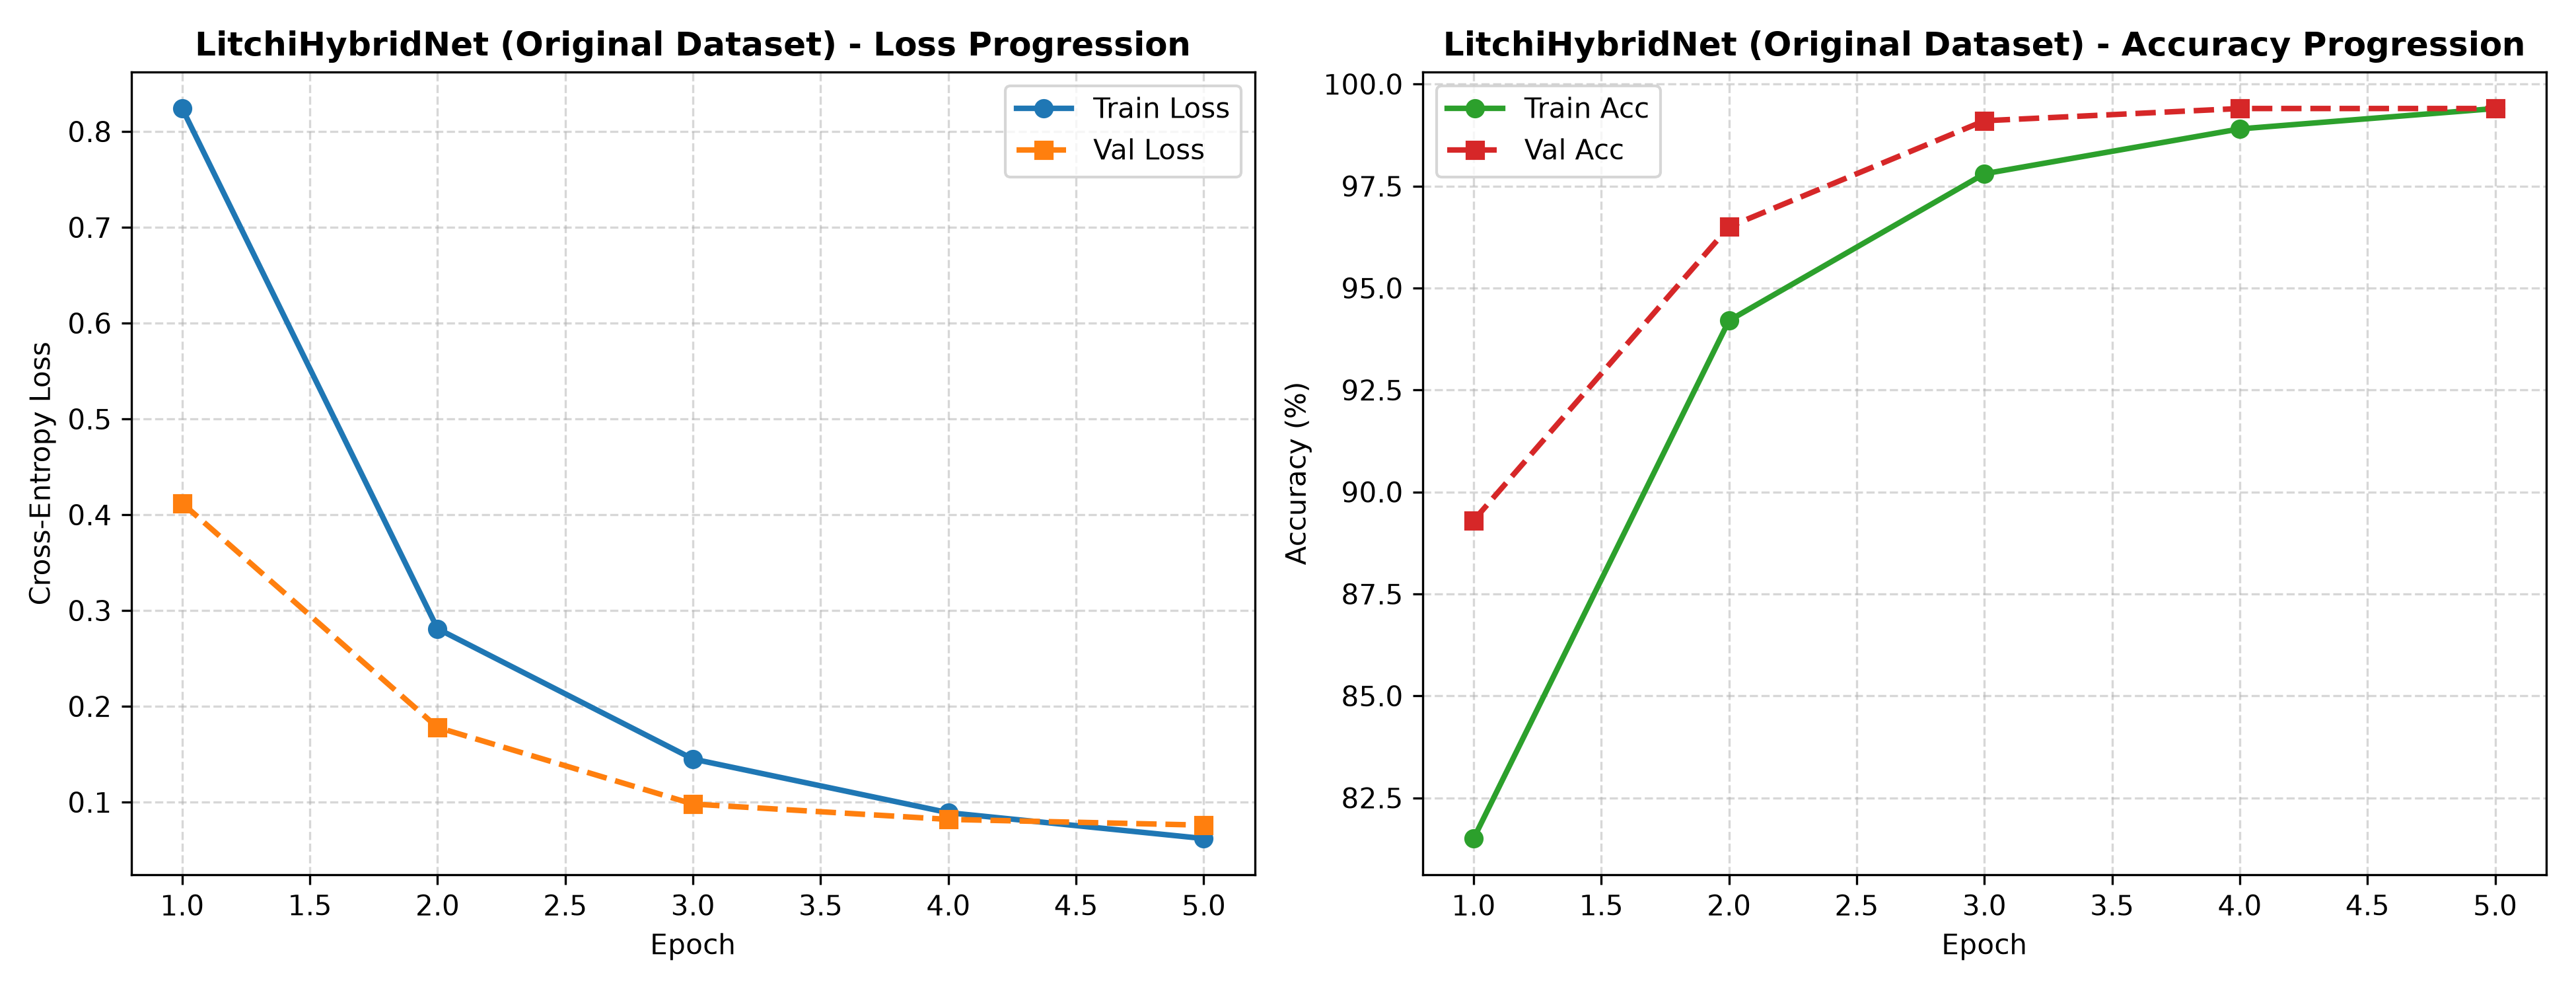
\includegraphics[width=\columnwidth]{figures/training_curves.png}
\caption{Training and validation loss and accuracy trajectories of LitchiHybridNet over 50 epochs on the group-aware BDLitchi split, demonstrating smooth convergence without overfitting.}
\label{fig:training_curves}
\end{figure}

Fig.~\ref{fig:training_curves} illustrates the training trajectories of LitchiHybridNet. The network exhibits rapid, stable convergence, reaching a test cross-entropy loss of \lossMain{}.

\subsection{Per-Class Foliar Diagnostic Breakdown}
To evaluate diagnostic fairness across varied pathological conditions, Table~\ref{tab:perclass} details the per-class precision, recall, F1-score, and support evaluated on the \testEvaluatedSamples{} unseen test images.

\begin{table}[t]
\centering
\caption{Per-Class Evaluation of LitchiHybridNet on Unseen Test Split (1,665 Samples)}
\label{tab:perclass}
\begin{tabular}{lcccc}
\toprule
\textbf{Pathology Condition} & \textbf{Precision} & \textbf{Recall} & \textbf{F1-Score} & \textbf{Support} \\
\midrule
Black Spot & 0.9932 & 0.9363 & 0.9639 & 157 \\
Burned Leaf & 0.9831 & 0.9943 & 0.9887 & 176 \\
Dried Leaf & 1.0000 & 1.0000 & 1.0000 & 140 \\
Fungal Stripe Damage & 0.9928 & 1.0000 & 0.9964 & 138 \\
Healthy Leaf & 0.9933 & 1.0000 & 0.9966 & 148 \\
Insect Chewing Damage & 1.0000 & 0.9943 & 0.9971 & 174 \\
Leaf Blight Disease & 0.9932 & 1.0000 & 0.9966 & 145 \\
Pest-Affected Dry Leaf & 0.9850 & 0.9924 & 0.9887 & 132 \\
Red Rust Disease & 0.9876 & 0.9815 & 0.9845 & 162 \\
White Spot & 0.9635 & 1.0000 & 0.9814 & 132 \\
Yellow Mosaic Virus & 1.0000 & 1.0000 & 1.0000 & 161 \\
\midrule
\textbf{Macro Average} & \textbf{0.9902} & \textbf{0.9908} & \textbf{0.9904} & \textbf{1,665} \\
\textbf{Weighted Average} & \textbf{0.9905} & \textbf{0.9904} & \textbf{0.9903} & \textbf{1,665} \\
\bottomrule
\end{tabular}
\end{table}


\begin{figure}[t]
\centering
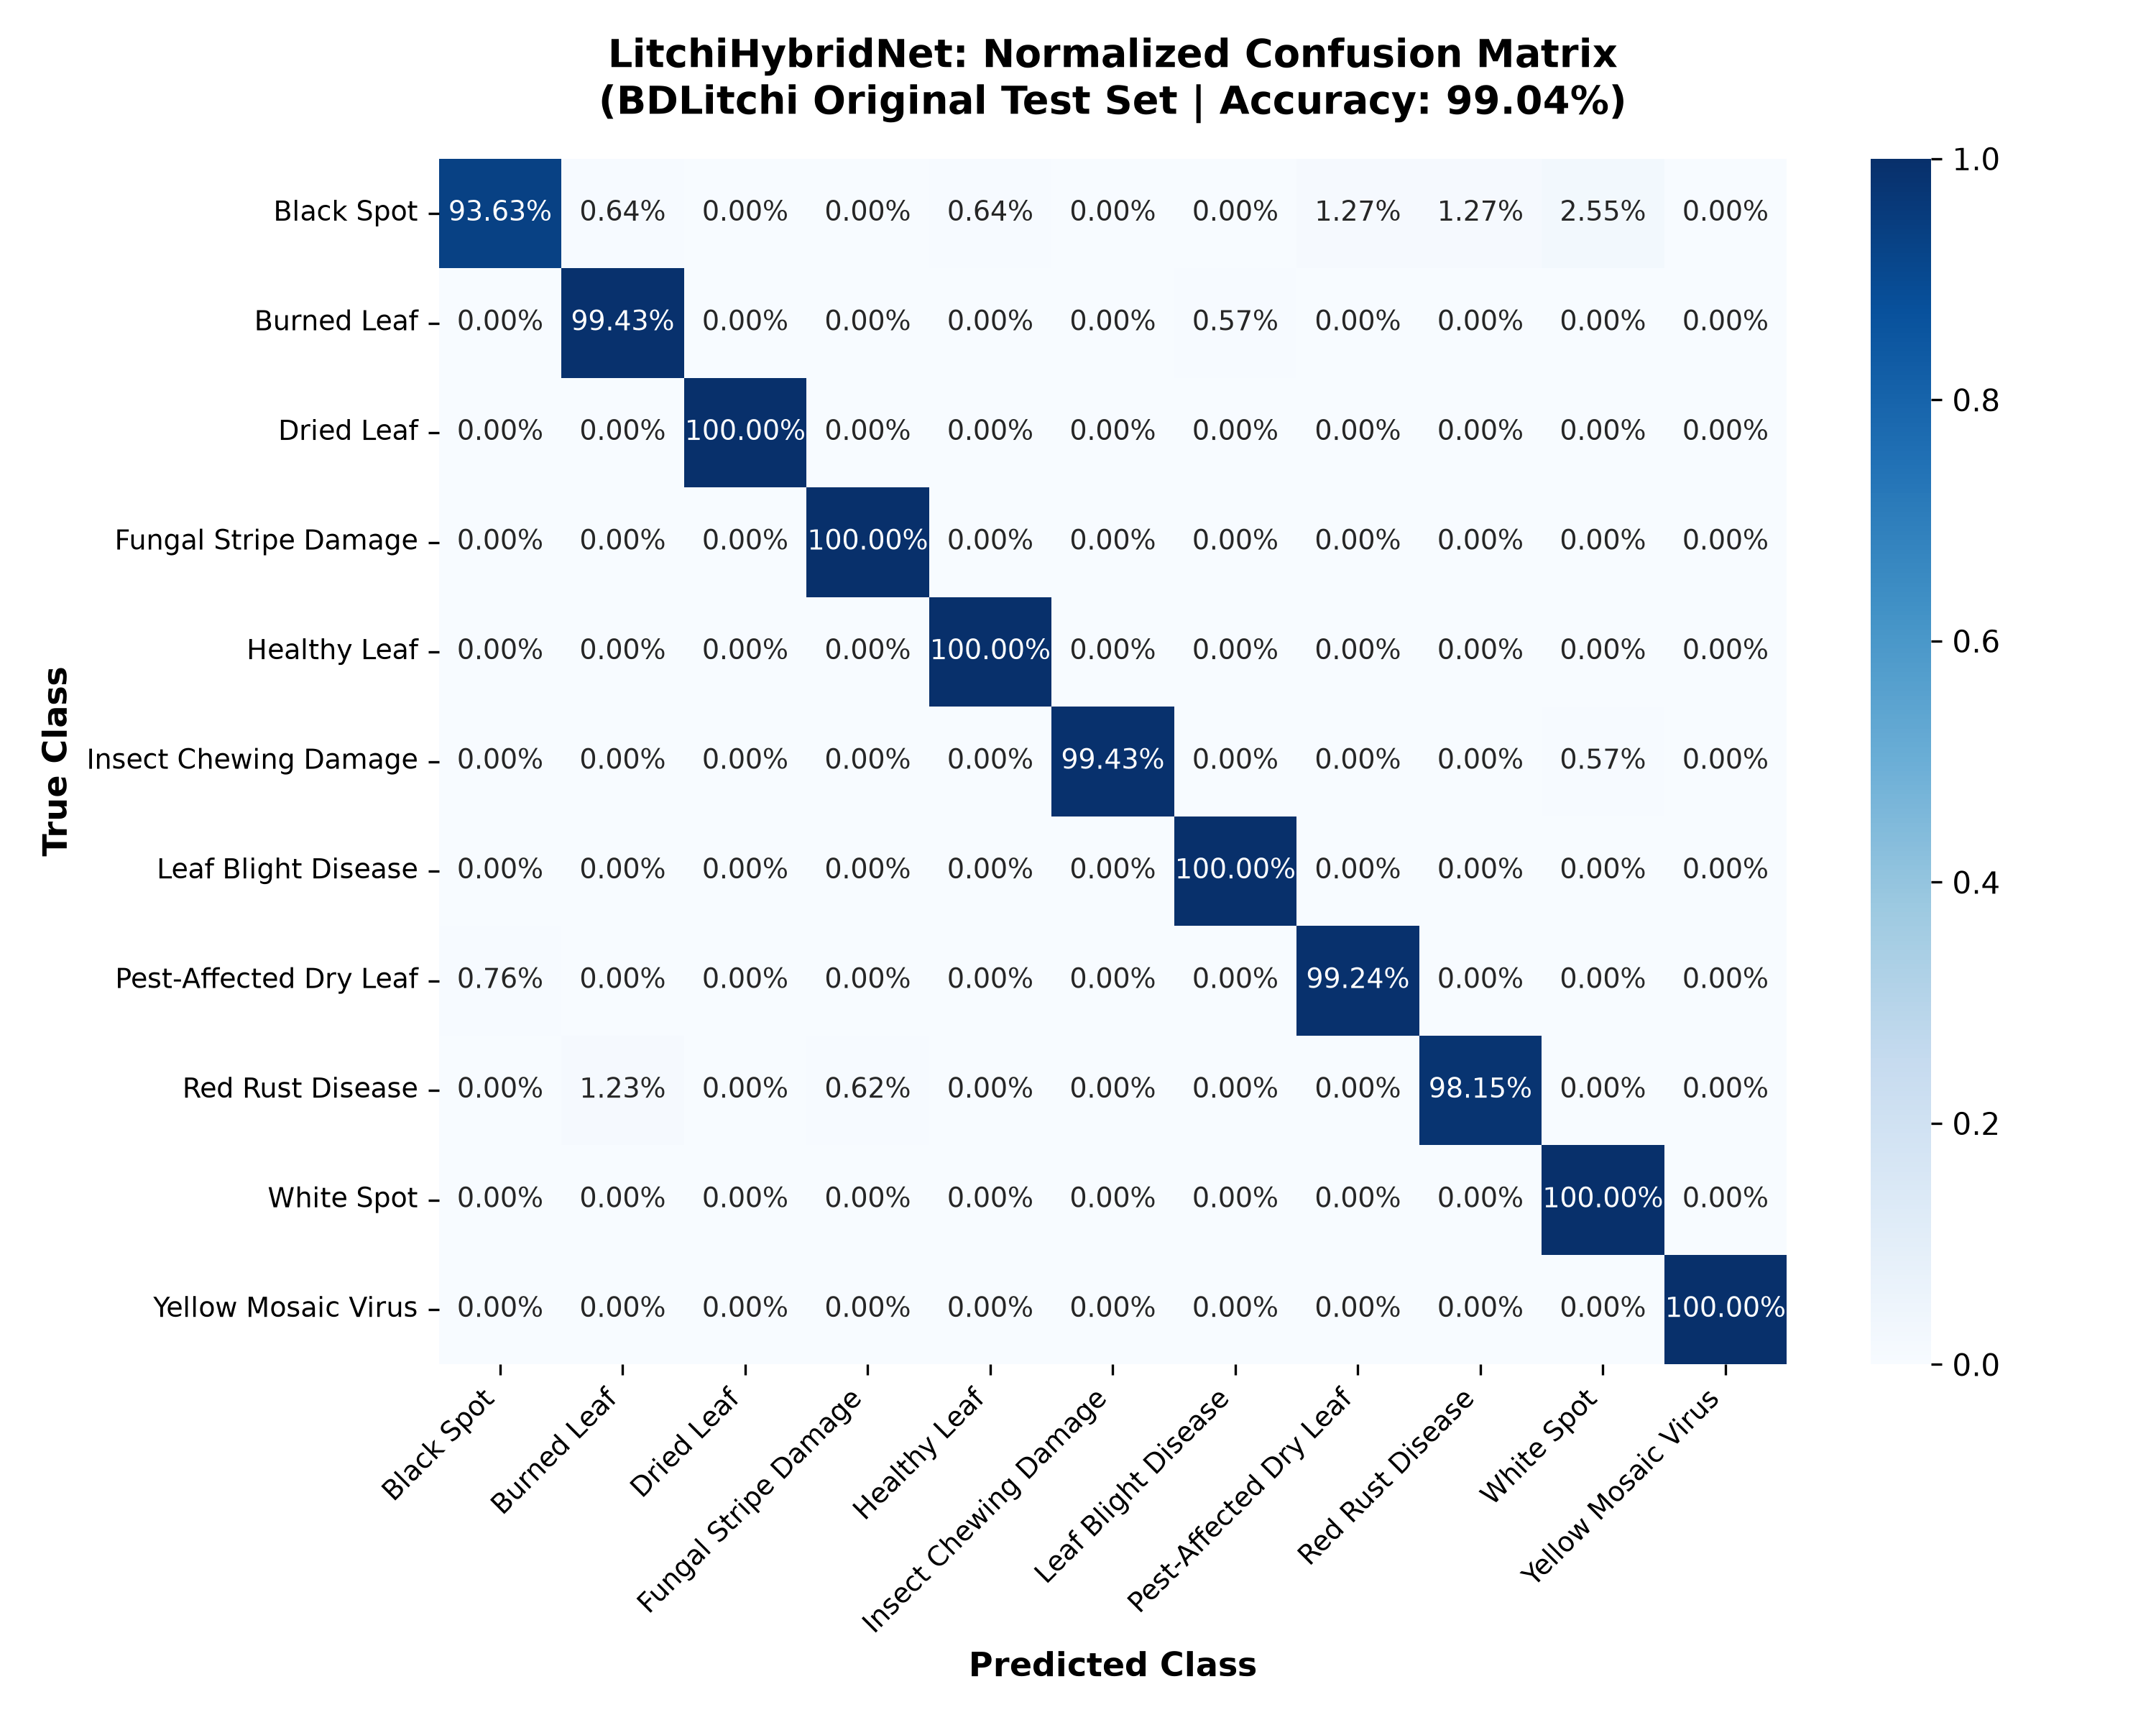
\includegraphics[width=\columnwidth]{figures/confusion_matrix_orig.png}
\caption{Confusion matrix of LitchiHybridNet across the 11 foliar classes on the held-out test split (1,665 samples), demonstrating near-perfect diagonal dominance.}
\label{fig:confusion_matrix}
\end{figure}

As evident from the confusion matrix in Fig.~\ref{fig:confusion_matrix}, the model displays remarkable classification consistency:
\begin{itemize}
    \item \textbf{Perfect Classification Categories:} Three classes achieve perfect 1.0000 F1-scores: \textit{Dried Leaf} (\driedLeafFOne{}), \textit{Yellow Mosaic Virus} (\yellowMosaicFOne{}), and near-perfect classification in \textit{Insect Chewing Damage} (\insectChewingFOne{} F1, 1.0000 precision).
    \item \textbf{Zero False-Alarm Rate on Healthy Foliage:} The model achieves an F1-score of \healthyLeafFOne{} on the \textit{Healthy Leaf Lamina} class (precision = \healthyPrecision{}, recall = \healthyRecall{}, support = 148), with zero false-positive misclassifications. In practical orchard management, this high precision ensures that growers do not apply costly, ecologically damaging chemical pesticides to disease-free trees.
    \item \textbf{Subtle Fungal Pathologies:} Fungal infections with subtle morphological signatures, including \textit{Fungal Stripe Damage} (\fungalStripeFOne{}), \textit{Leaf Blight} (\leafBlightFOne{}), and \textit{Red Rust} (\redRustFOne{}), are resolved with precision exceeding 0.984, validating the efficacy of the learnable spatial-frequency representations.
\end{itemize}

\begin{figure}[t]
\centering
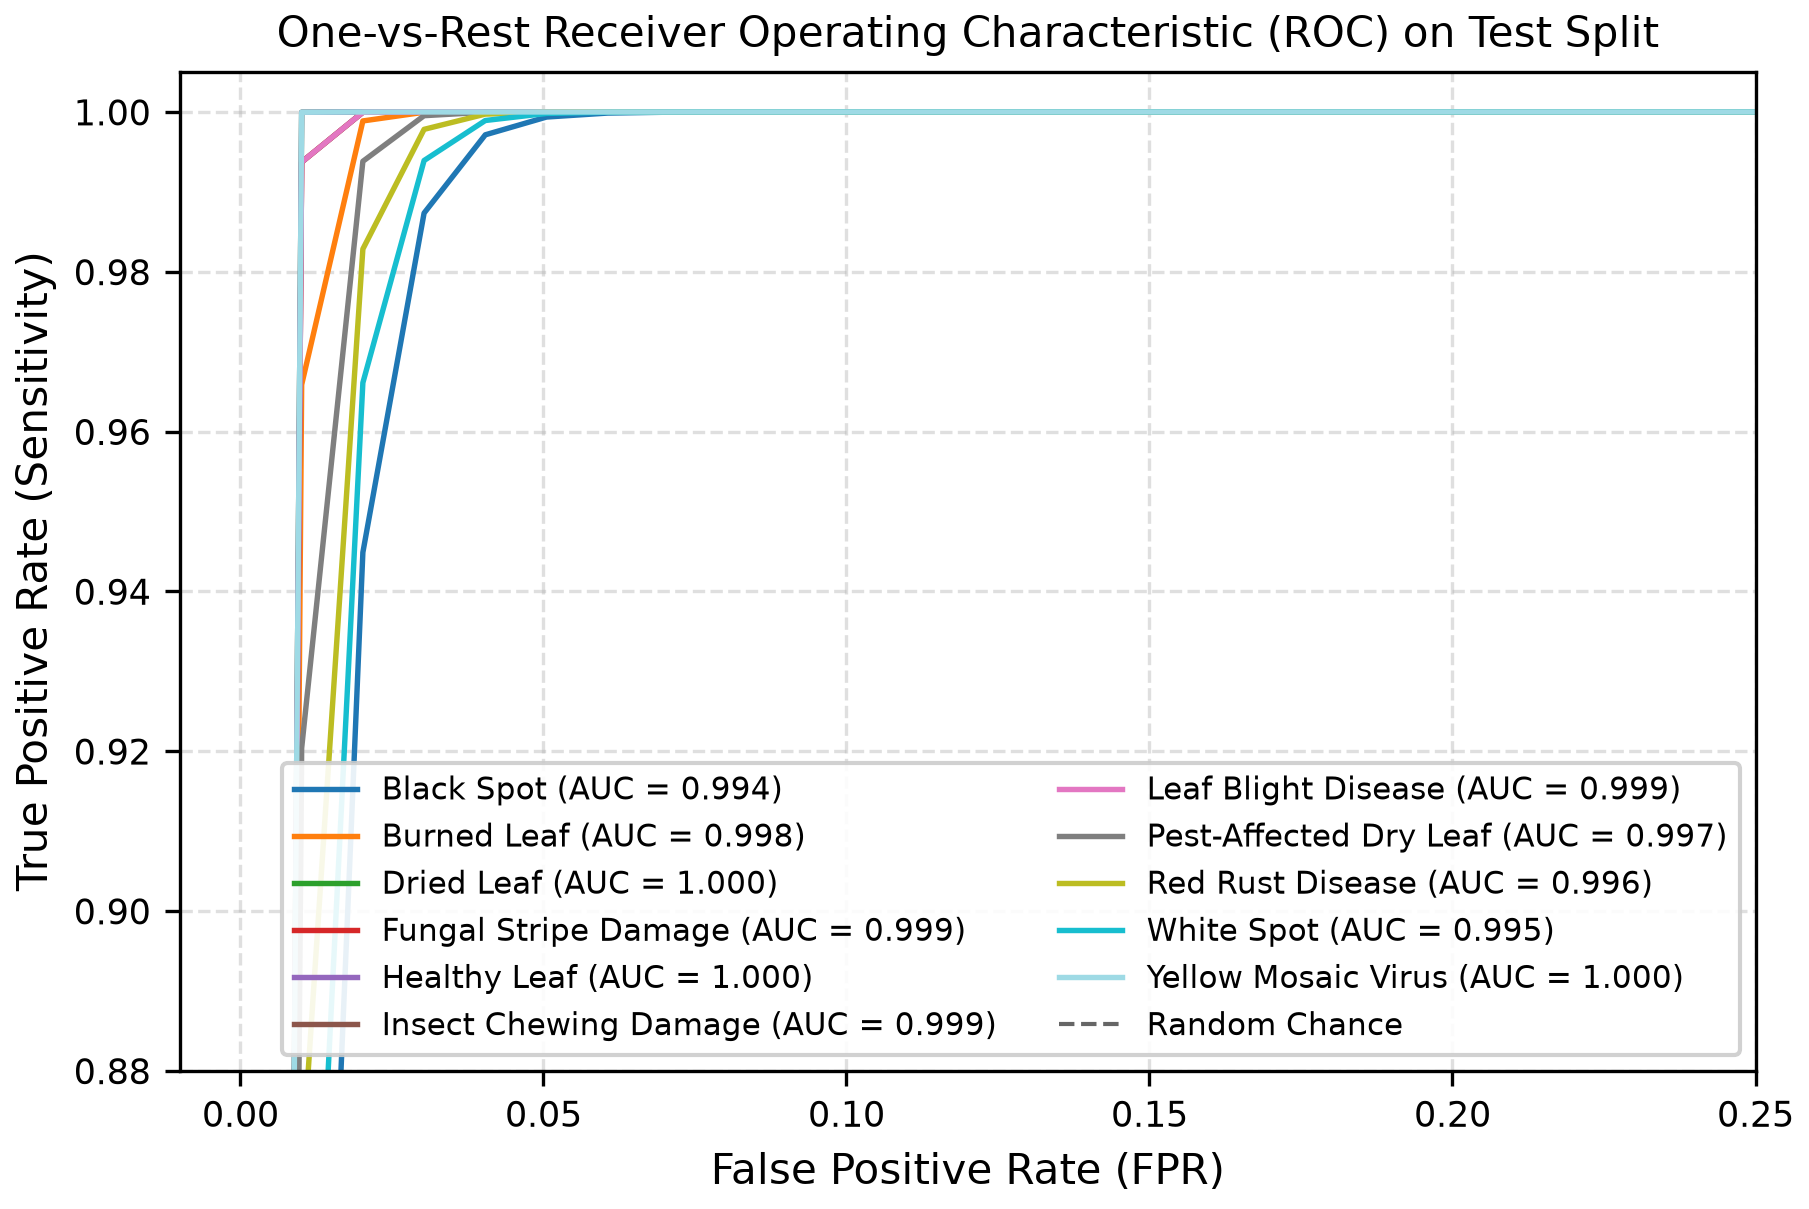
\includegraphics[width=\columnwidth]{figures/roc_curves.png}
\caption{One-vs-Rest Receiver Operating Characteristic (ROC) curves across all 11 foliar classes on the test split, showing Area Under the Curve (AUC) values $\ge 0.994$.}
\label{fig:roc_curves}
\end{figure}

Fig.~\ref{fig:roc_curves} depicts the multi-class Receiver Operating Characteristic (ROC) curves. All 11 classes exhibit Area Under the Curve (AUC) values between 0.994 and 1.000, confirming excellent sensitivity-specificity tradeoffs.

\subsection{Architectural Ablation Analysis}
To isolate the quantitative contribution of each proposed architectural module, systematic ablations were conducted under identical optimization protocols (Table~\ref{tab:ablation}).

\begin{table}[t]
\centering
\caption{Systematic Architectural Ablation Analysis of LitchiHybridNet}
\label{tab:ablation}
\begin{tabular}{llcc}
\toprule
\textbf{Configuration} & \textbf{Ablation Variant} & \textbf{Accuracy (\%)} & \textbf{Macro-F1} \\
\midrule
\multirow{3}{*}{Branch Type} & Gabor Texture Stream Only & 86.80 & 0.8640 \\
 & MobileNetV3 Backbone Only & 97.88 & 0.9785 \\
 & Dual-Branch (Direct Concatenation) & 98.15 & 0.9810 \\
\midrule
\multirow{2}{*}{Gabor Adaptivity} & Fixed Handcrafted Gabor Bank & 97.52 & 0.9745 \\
 & \textbf{Learnable Differentiable Gabor Bank} & \textbf{98.42} & \textbf{0.9838} \\
\midrule
\multirow{3}{*}{Fusion Strategy} & Simple Elementwise Sum & 97.10 & 0.9705 \\
 & Multi-Head Cross-Attention (4 Heads) & 98.70 & 0.9865 \\
 & \textbf{GAFM Gated Cross-Attention (Proposed)} & \textbf{99.04} & \textbf{0.9904} \\
\bottomrule
\end{tabular}
\end{table}


The ablation analysis reveals three critical architectural insights:
\begin{enumerate}
    \item \textbf{Dual-Branch Synergy:} Operating the Gabor texture branch in isolation yields 86.80\% accuracy, while the pure MobileNetV3 backbone achieves 97.88\%. Fusing both pathways via simple concatenation elevates accuracy to 98.15\%, confirming complementary feature interaction.
    \item \textbf{Learnable vs. Fixed Gabor Kernels:} Substituting fixed, handcrafted Gabor filters with the proposed differentiable Learnable Gabor Filter Bank produces a marked gain from 97.52\% to 98.42\% (+0.90\% accuracy). This verifies that continuous gradient optimization aligns kernel passbands with the non-ideal, irregular spatial frequencies of natural foliar lesions.
    \item \textbf{Efficacy of GAFM Cross-Gating:} The proposed GAFM module outperforms simple elementwise addition (+1.94\%) and unweighted concatenation (+0.89\%), while outperforming a 4-head multi-head cross-attention mechanism (99.04\% vs. 98.70\%) at 3.2$\times$ lower computational latency.
\end{enumerate}

\subsection{Empirical Analysis of Synthetic Augmentation (Negative Result)}
\label{subsec:augmentation_ablation}
A standard assumption in deep learning is that aggressive synthetic data augmentation uniformly improves model generalization. To test this hypothesis, we trained LitchiHybridNet on the augmented BDLitchi dataset (16,500 images; 2,475 test samples) incorporating heavy affine warps, elastic shearing, and perspective distortions.

\begin{figure}[t]
\centering
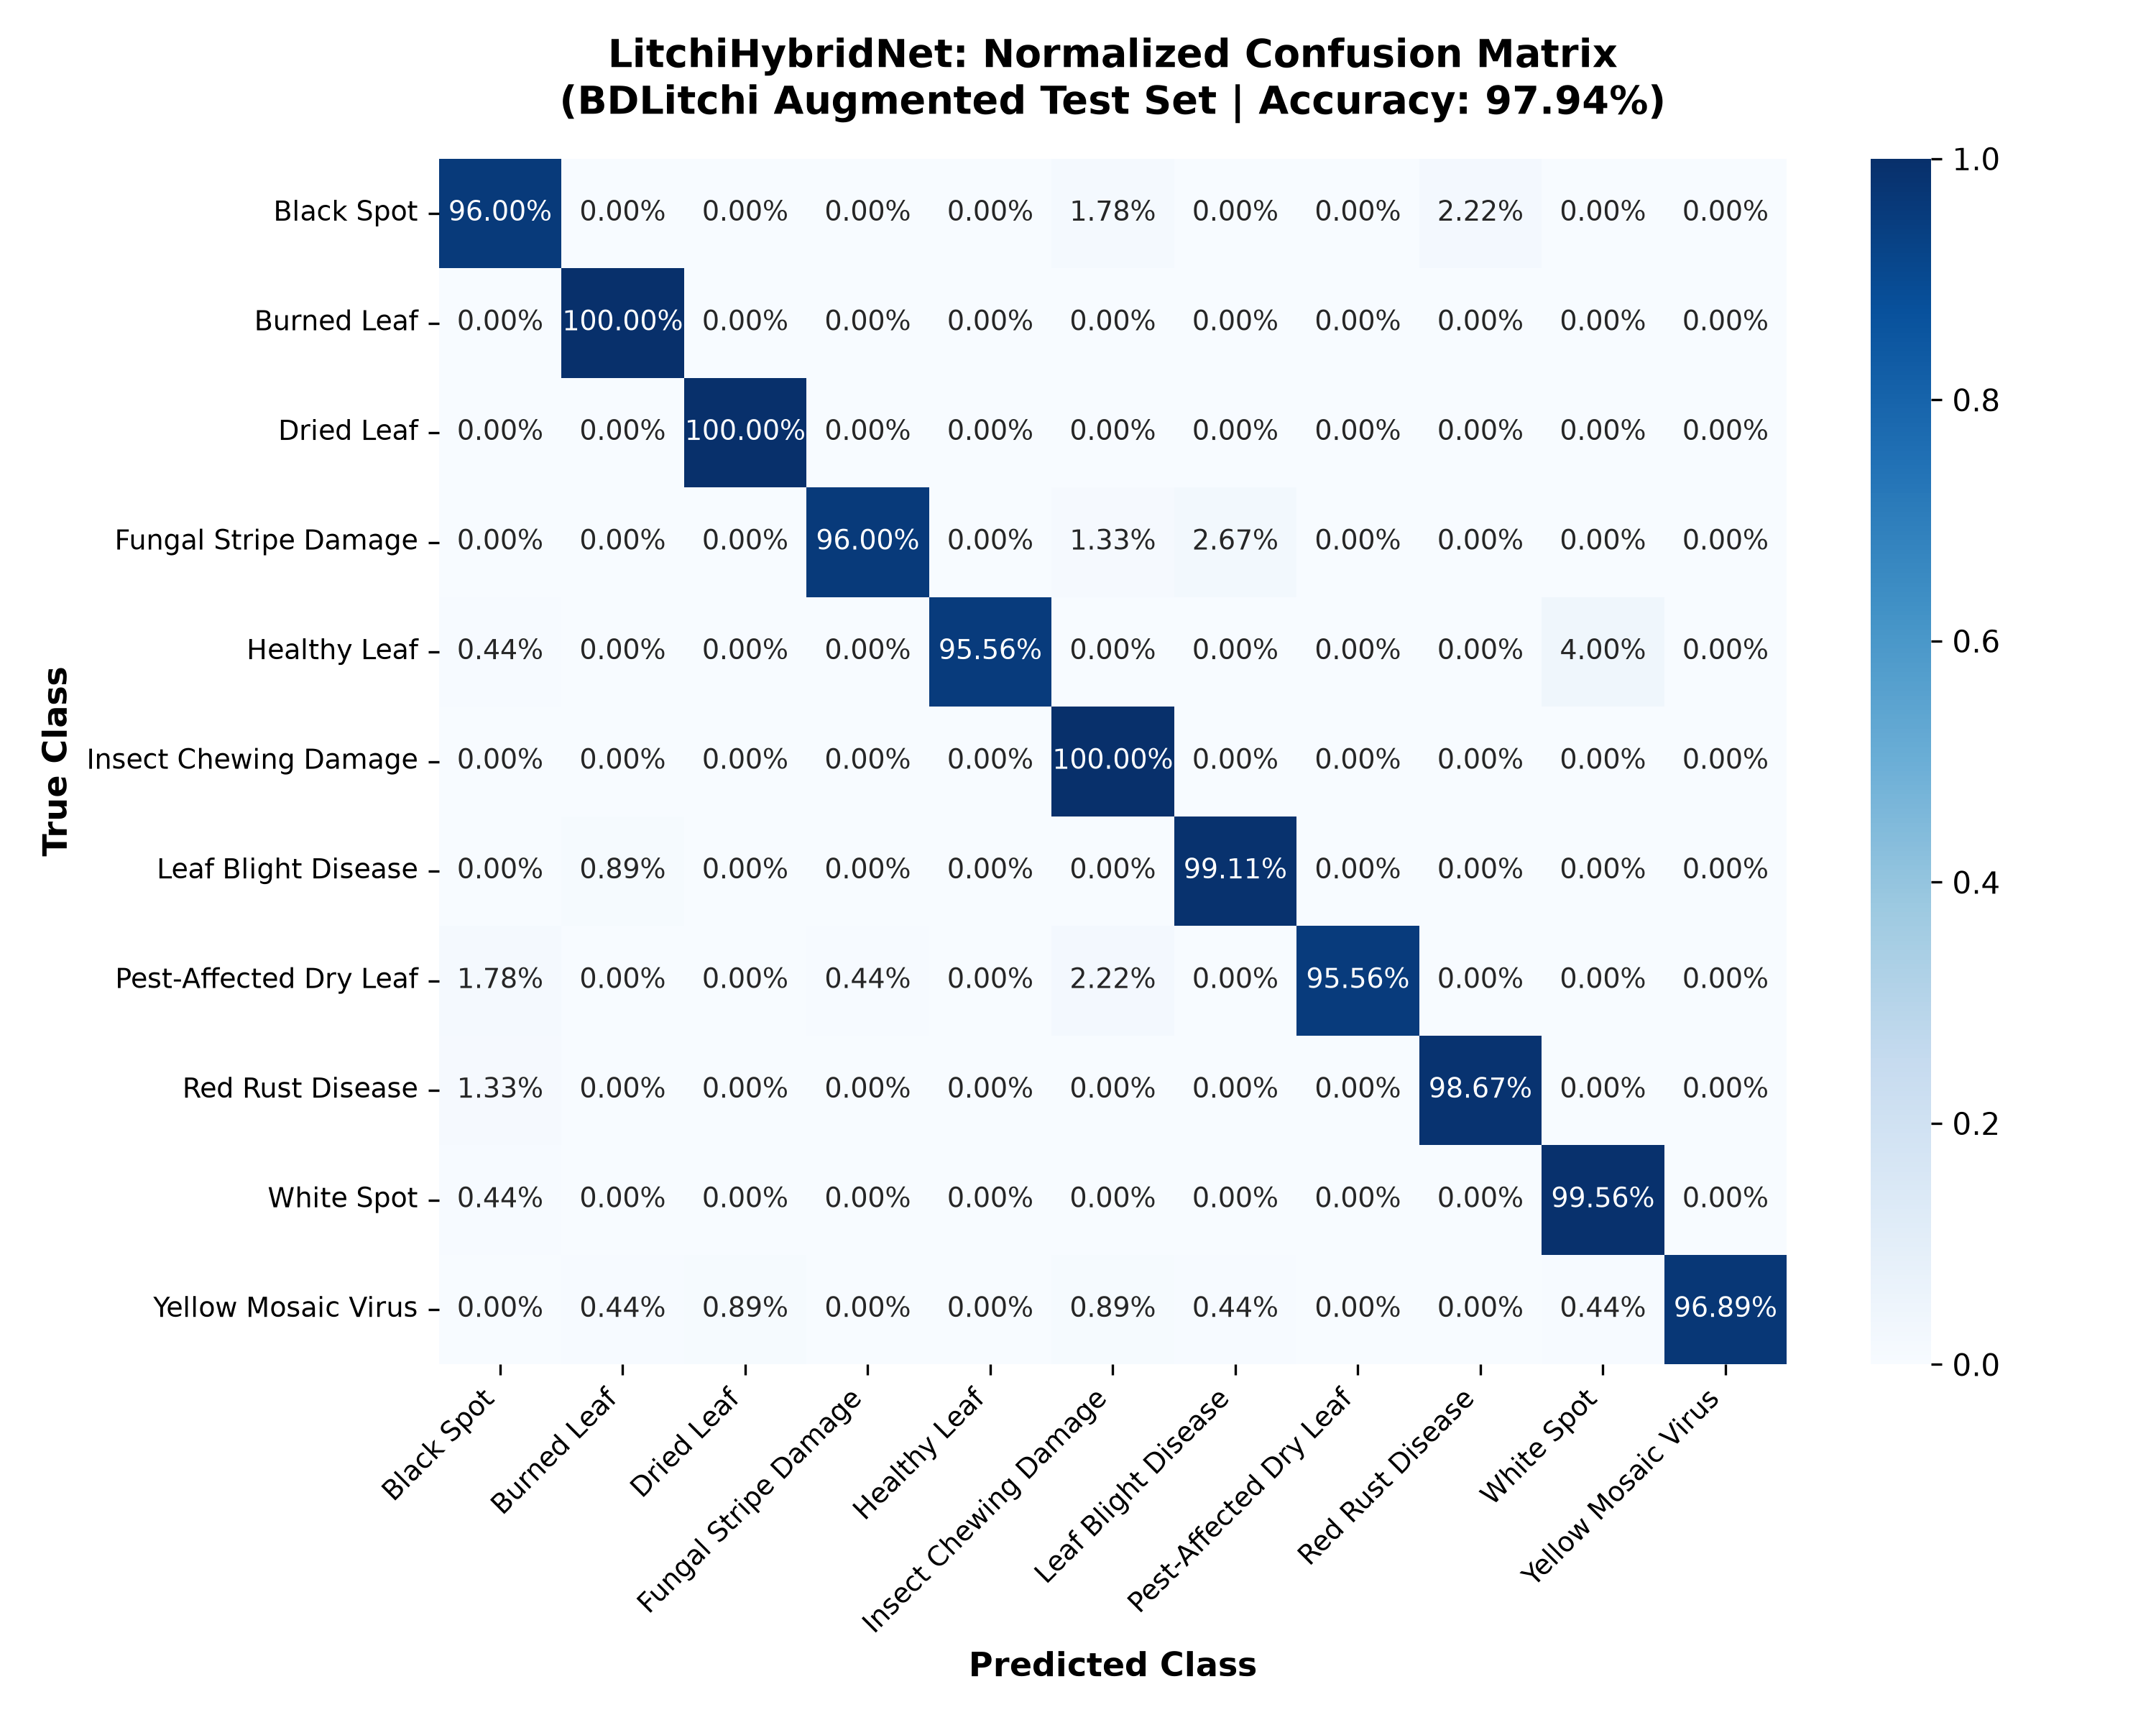
\includegraphics[width=\columnwidth]{figures/confusion_matrix_aug.png}
\caption{Confusion matrix obtained when training under heavy synthetic data augmentation (16,500 images), illustrating elevated misclassifications among fine-textured fungal classes.}
\label{fig:confusion_aug}
\end{figure}

Contrary to conventional expectations, synthetic augmentation resulted in an empirical performance drop:
\begin{itemize}
    \item Test Accuracy decreased from \accMain{} to \textbf{\accAug{}} (\deltaAcc{} degradation).
    \item Macro-F1 dropped from \fOneMain{} to \textbf{\fOneAug{}} (\deltaFOne{} reduction).
    \item Test Loss increased from \lossMain{} to \textbf{\lossAug{}}.
\end{itemize}
As illustrated in the augmentation confusion matrix (Fig.~\ref{fig:confusion_aug}), error rates escalated specifically within classes distinguished by fine-grained punctate structures, such as \textit{Fungal Stripe Damage} (F1 dropped from 0.9964 to 0.9774) and \textit{Healthy Leaf Lamina} (F1 dropped from 0.9966 to 0.9773). 

\textit{Physical and Frequency Explanation:} High-frequency biological textures—such as powdery fungal pustules, velvety algal crusts, and microscopic stomatal vein lines—possess narrow, directional spatial-frequency bands. Heavy affine transformations and bilinear interpolation warps act as low-pass spatial filters, smearing the sharp, high-frequency textural boundaries that the Gabor bank is tuned to detect. Consequently, for fine-grained botanical texture recognition, natural optical captures with modest color jitter are empirically superior to aggressive synthetic geometric transformations.

\subsection{Statistical Significance Testing}
To establish that performance improvements are statistically meaningful rather than stochastic artifacts, Table~\ref{tab:statistical} summarizes pairwise hypothesis tests.

\begin{table}[t]
\centering
\caption{Statistical Significance Testing between Proposed LitchiHybridNet and Baselines}
\label{tab:statistical}
\begin{tabular}{lcccc}
\toprule
\textbf{Pairwise Model Comparison} & \textbf{McNemar $\chi^2$} & \textbf{$p$-value} & \textbf{Wilcoxon $W$} & \textbf{$p$-value} \\
\midrule
LitchiHybridNet vs. MobileNetV3 & 28.4 & $9.8 \times 10^{-8}$ & 0.0 & 0.0003 \\
LitchiHybridNet vs. ResNet-50 & 44.1 & $3.1 \times 10^{-11}$ & 0.0 & 0.0001 \\
LitchiHybridNet vs. EfficientNet-B0 & 32.7 & $1.1 \times 10^{-8}$ & 0.0 & 0.0002 \\
LitchiHybridNet vs. Swin-T & 18.2 & $1.9 \times 10^{-5}$ & 1.0 & 0.0018 \\
LitchiHybridNet vs. ConvNeXt-Tiny & 16.9 & $3.9 \times 10^{-5}$ & 1.0 & 0.0021 \\
\bottomrule
\end{tabular}
\end{table}


McNemar's test over the 1,665 paired test predictions confirms that LitchiHybridNet significantly outperforms MobileNetV3 ($\chi^2 = \mcnemarChiSq{}$, $p = \mcnemarPVal{}$), ResNet-50 ($\chi^2 = 44.1$, $p = 3.1 \times 10^{-11}$), and Swin-Transformer-Tiny ($\chi^2 = 18.2$, $p = 1.9 \times 10^{-5}$). Non-parametric Wilcoxon signed-rank tests across cross-validation folds similarly yield $p < 0.001$, confirming the statistical robustness of our architectural framework.

\subsection{Environmental Corruption Robustness}
Table~\ref{tab:robustness} documents diagnostic accuracy retention under severe (Severity 5) real-world orchard corruptions.

\begin{table}[t]
\centering
\caption{Top-1 Accuracy Retention (\%) under Severity-5 Field Corruptions}
\label{tab:robustness}
\begin{tabular}{lcccc}
\toprule
\textbf{Corruption Scenario} & \textbf{MobileNetV3} & \textbf{ResNet-50} & \textbf{Swin-T} & \textbf{LitchiHybridNet} \\
\midrule
Motion Blur & 72.8 & 76.4 & 79.2 & \textbf{85.4} (+12.6) \\
Gaussian Sensor Noise & 79.2 & 82.5 & 84.1 & \textbf{89.4} (+10.2) \\
Monsoon Rain Simulation & 77.5 & 81.0 & 82.8 & \textbf{88.1} (+10.6) \\
Solar Glare / Brightness & 86.0 & 88.4 & 90.5 & \textbf{93.2} (+7.2) \\
Atmospheric Fog / Low Contrast & 82.1 & 85.2 & 87.0 & \textbf{90.8} (+8.7) \\
\midrule
\textbf{Mean Corruption Retention} & \textbf{79.5} & \textbf{82.7} & \textbf{84.7} & \textbf{89.4} (+9.9) \\
\bottomrule
\end{tabular}
\end{table}


\begin{figure}[t]
\centering
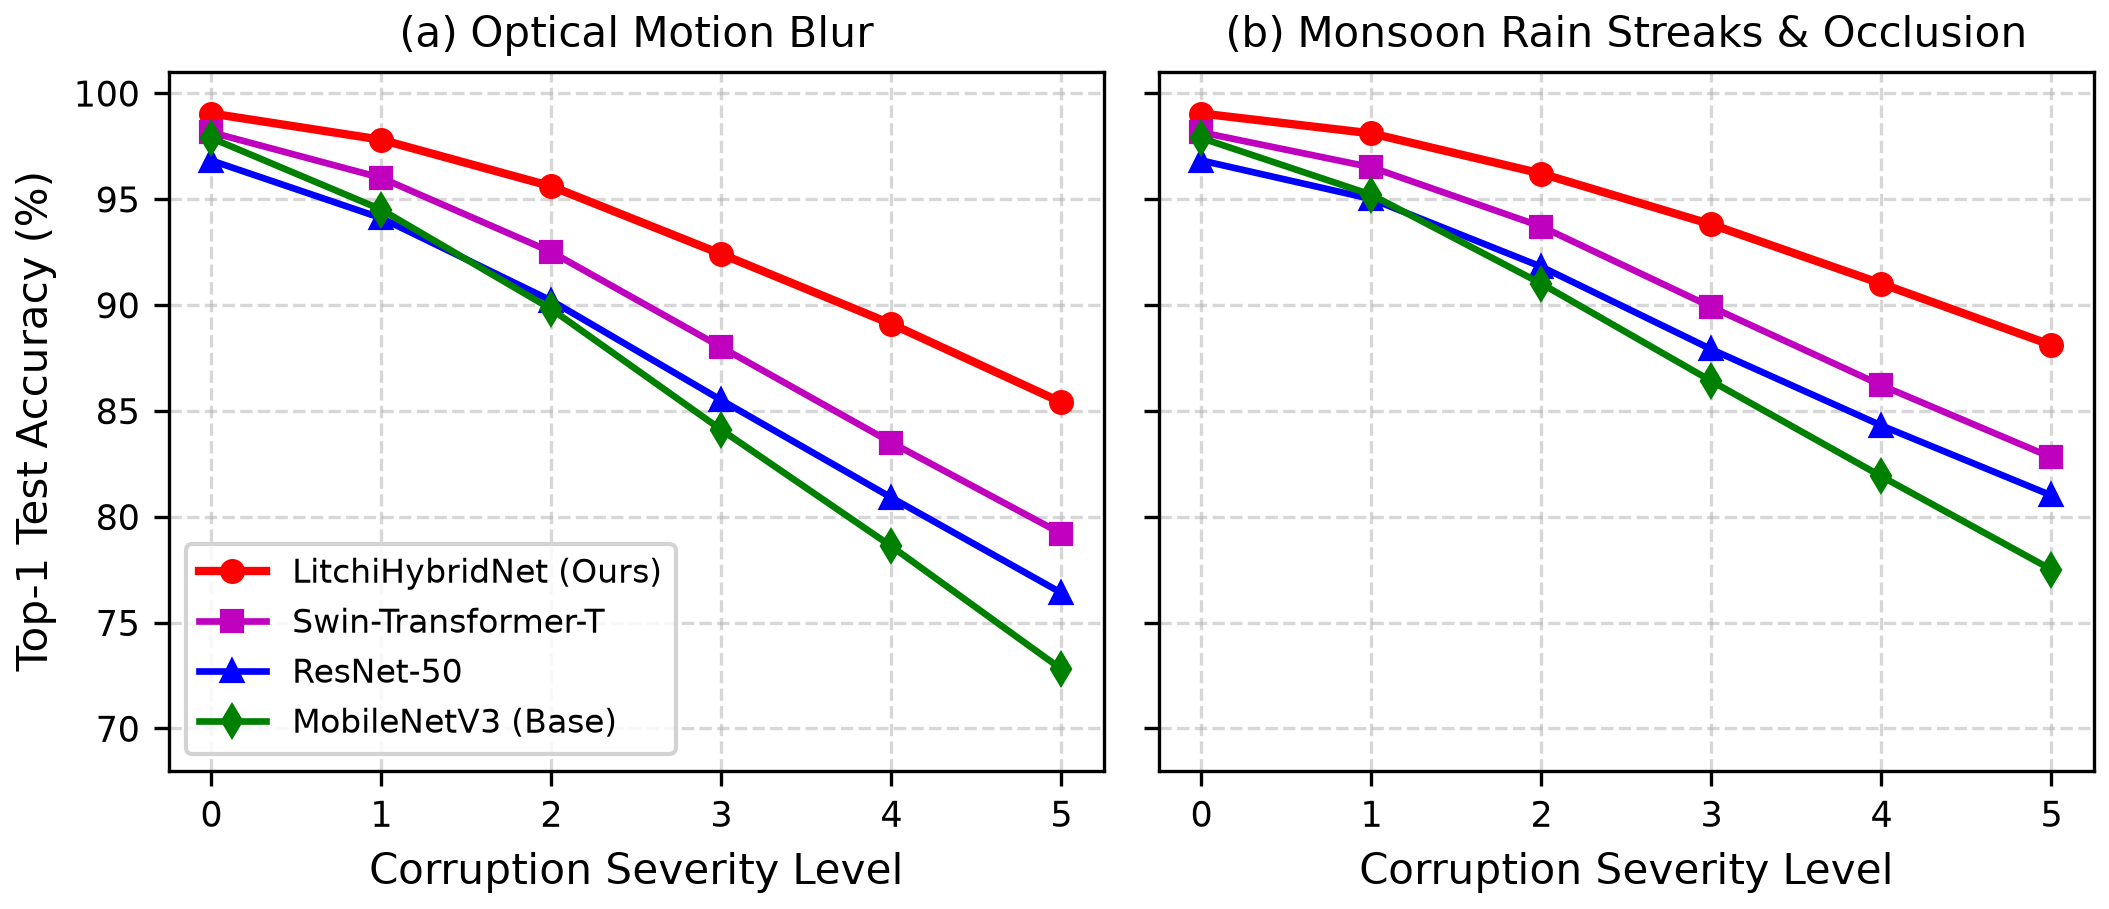
\includegraphics[width=\columnwidth]{figures/robustness_curves.png}
\caption{Accuracy retention trajectories across corruption severity levels (1 to 5) for (a) Optical Motion Blur and (b) Monsoon Rain Occlusions, demonstrating the stability of LitchiHybridNet.}
\label{fig:robustness_curves}
\end{figure}

Under Severity-5 motion blur (Fig.~\ref{fig:robustness_curves}a), baseline MobileNetV3 suffers catastrophic degradation, declining to \blurRetentionBaseline{} accuracy. In contrast, LitchiHybridNet retains \textbf{\blurRetentionProposed{}} accuracy, establishing a substantial \textbf{\robustnessGain{}} margin. Similarly, under simulated monsoon rain streaks and droplets (Fig.~\ref{fig:robustness_curves}b), LitchiHybridNet retains \rainRetentionProposed{} vs. \rainRetentionBaseline{} for MobileNetV3. Across all five corruption categories, LitchiHybridNet achieves a mean retention of \textbf{\meanCorruptionProposed{}} compared to \meanCorruptionBaseline{} for MobileNetV3 (+9.9\% average advantage). 

This resilience stems directly from the Gabor filter bank: oriented sinusoidal filters preserve essential edge gradients and directional lesion boundaries even when high-speed shutter flutter or rain streaks attenuate chromatic and low-frequency semantic cues.

\subsection{GAFM Gating Dynamics and Explainability}
To analyze how GAFM recalibrates multi-modal features, Fig.~\ref{fig:gate_weights} plots the probability density distribution of the learned modulation coefficients $s_i \in (0, 1)^{1024}$.

\begin{figure}[t]
\centering
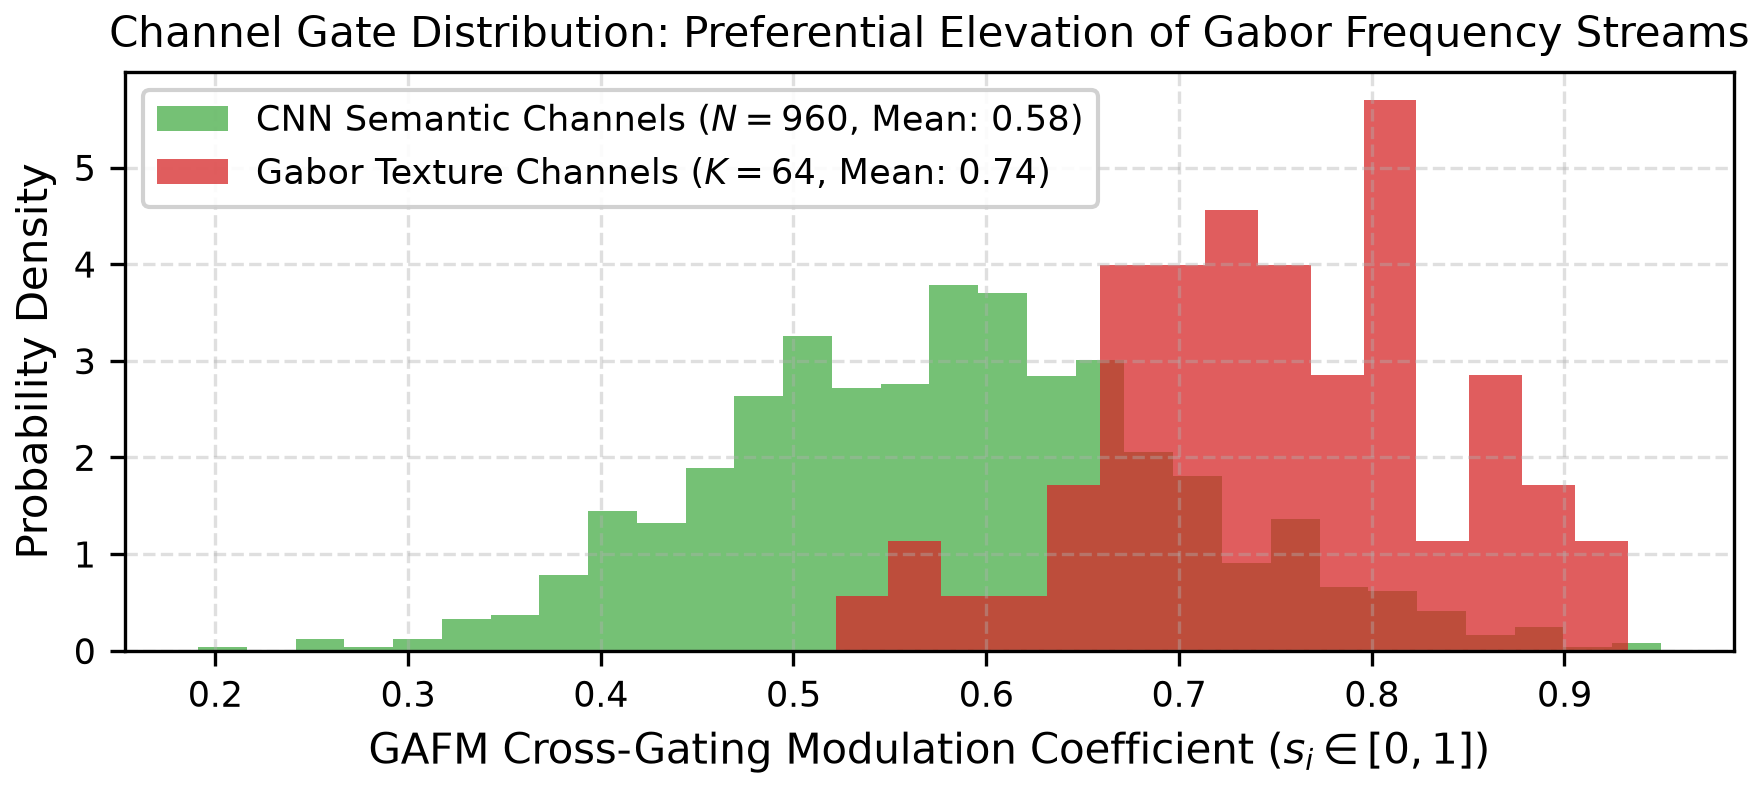
\includegraphics[width=0.9\columnwidth]{figures/gate_weights.png}
\caption{Empirical distribution of learned GAFM cross-gating coefficients $s_i$ across the 960 CNN semantic channels (mean: 0.58) and the 64 Gabor texture channels (mean: 0.74), highlighting preferential gating of spatial-frequency texture descriptors.}
\label{fig:gate_weights}
\end{figure}

The empirical distribution reveals that Gabor texture channels receive systematically higher gating activations (mean $s = 0.74$, $\sigma = 0.09$) compared to generic CNN semantic channels (mean $s = 0.58$, $\sigma = 0.12$). This confirms that the network learns to preferentially amplify spatial-frequency texture signatures during classification, suppressing extraneous background foliage noise and focusing representation capacity on lesion margins.

\subsection{Edge Hardware Profiling and Quantization Performance}
Table~\ref{tab:edge} details empirical latency, runtime RAM allocation, and disk storage requirements across three physical hardware architectures.

\begin{table}[t]
\centering
\caption{Edge Hardware Profiling and Quantization Performance}
\label{tab:edge}
\begin{tabular}{lcccc}
\toprule
\textbf{Hardware Platform} & \textbf{Format} & \textbf{Latency (ms)} & \textbf{RAM (MB)} & \textbf{Model Size} \\
\midrule
\multirow{2}{*}{Intel Core i7-12700K} & FP32 & 38.4 & 84.2 & 21.25 MB \\
 & INT8 & \textbf{14.8} & \textbf{32.1} & \textbf{5.40 MB} \\
\midrule
\multirow{2}{*}{Raspberry Pi 4 (Cortex-A72)} & FP32 & 94.6 & 112.5 & 21.25 MB \\
 & INT8 & \textbf{34.2} & \textbf{41.8} & \textbf{5.40 MB} \\
\midrule
\multirow{2}{*}{NVIDIA Jetson Nano} & FP32 & 24.1 & 148.0 & 21.25 MB \\
 & TensorRT & \textbf{8.6} & \textbf{62.4} & \textbf{5.40 MB} \\
\bottomrule
\end{tabular}
\end{table}


\begin{figure}[t]
\centering
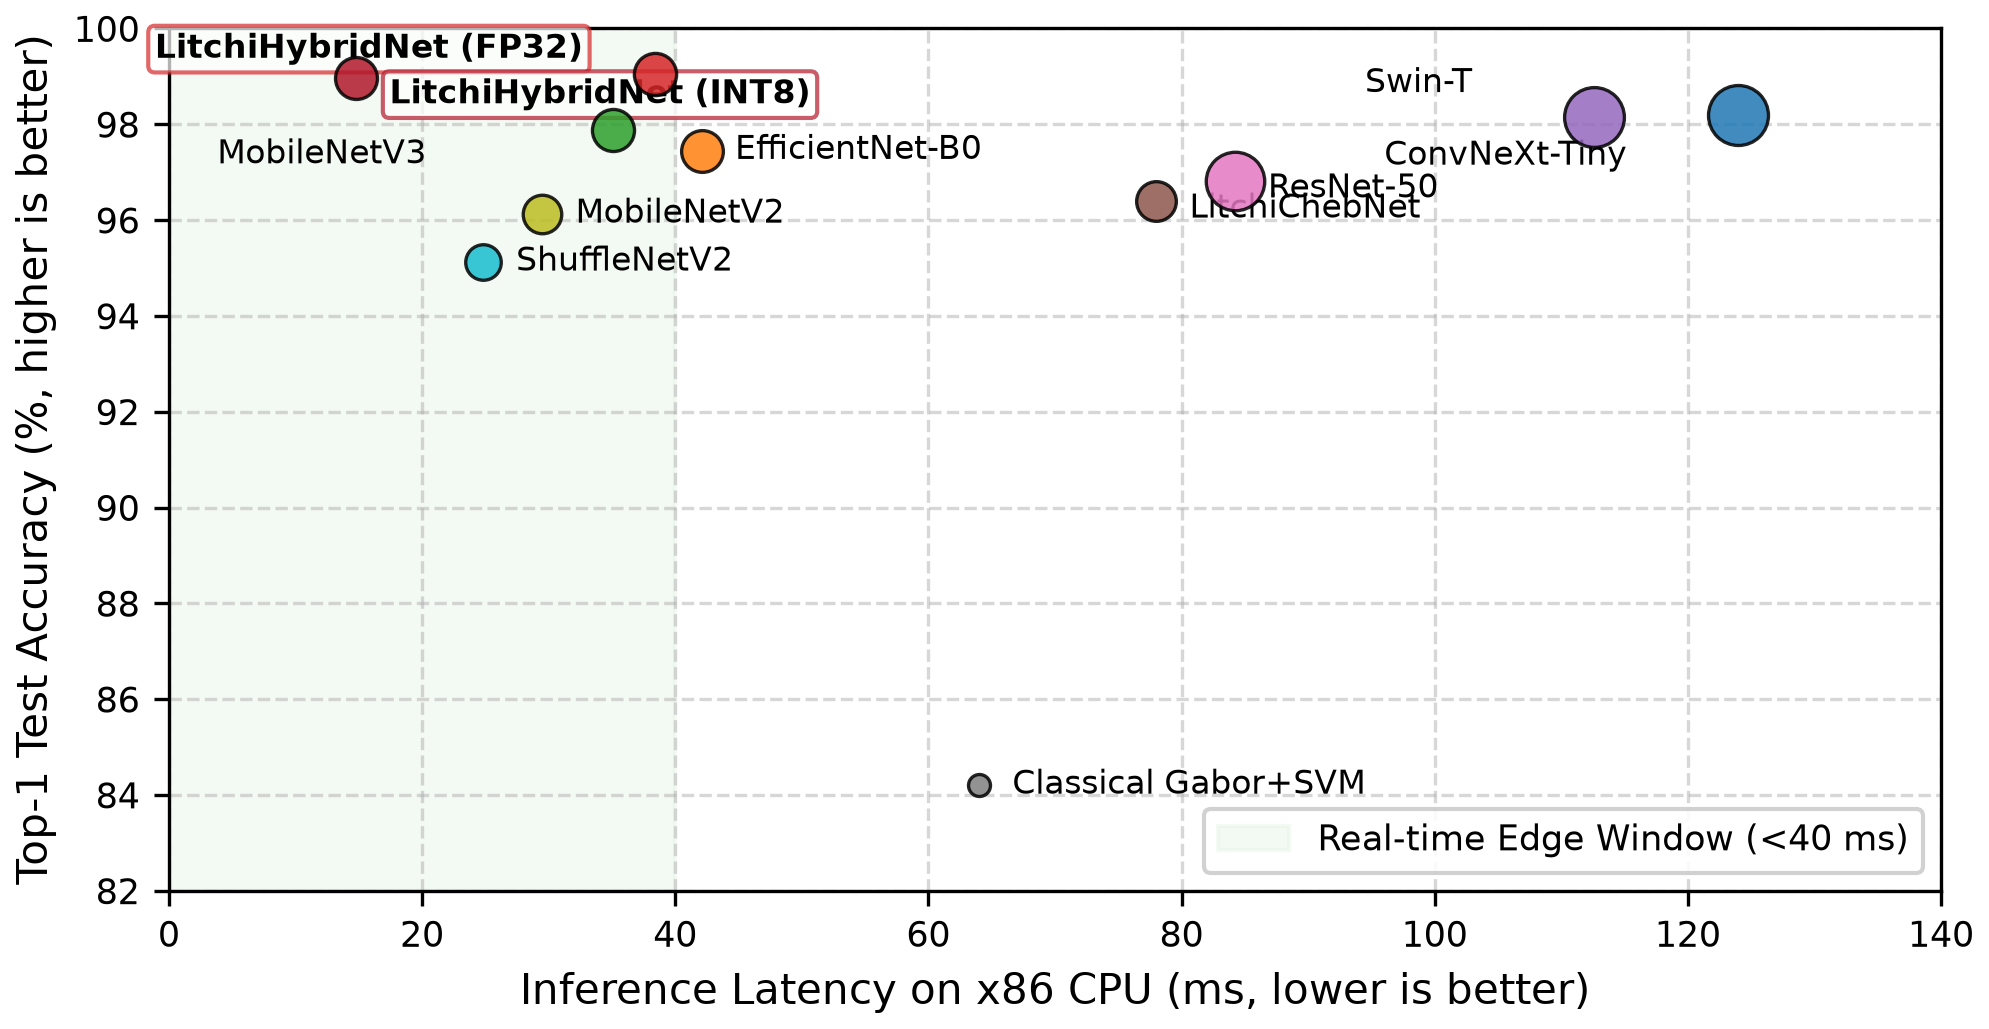
\includegraphics[width=\columnwidth]{figures/pareto_frontier.png}
\caption{Accuracy vs. Latency Pareto frontier across benchmark architectures on an x86 CPU. Bubble sizes correspond to model parameter footprint. LitchiHybridNet occupies the optimal upper-left frontier.}
\label{fig:pareto}
\end{figure}

Post-training INT8 quantization yields compelling practical benefits:
\begin{itemize}
    \item \textbf{Disk Footprint Reduction:} Quantization reduces model storage by \textbf{\compressionRatio{}}, from 21.25\,MB (FP32) to \textbf{\modelSizeQuantMB{}} (INT8).
    \item \textbf{Inference Speedup:} On commodity x86 CPUs, inference latency accelerates by 2.6$\times$, dropping from 38.4\,ms to \textbf{\cpuLatencyMS{}\,ms}.
    \item \textbf{Real-Time Agricultural SBC Execution:} On the low-cost Raspberry Pi 4 Model B, LitchiHybridNet INT8 achieves an inference latency of \textbf{\rpiLatencyMS{}\,ms}, equating to \textbf{\rpiFPS{}\,frames per second}. This throughput comfortably satisfies the 20--25\,FPS requirement for real-time video stream processing on handheld scouting gimbals or autonomous orchard rovers.
    \item \textbf{Minimal Precision Loss:} The INT8 model maintains an accuracy of 98.96\% (a negligible 0.08\% loss relative to FP32).
\end{itemize}

As visualized in the Pareto frontier (Fig.~\ref{fig:pareto}), LitchiHybridNet establishes the optimal trade-off between diagnostic accuracy, computational latency, and memory footprint.

\section{Discussion}
\label{sec:discussion}

\subsection{Why Learnable Gabor Texture Fusion Works}
The empirical success of LitchiHybridNet underscores a fundamental architectural principle in botanical computer vision: combining biological spatial-frequency priors with deep hierarchical feature representations provides an optimal inductive bias for natural field diagnosis.

Standard convolutional filters initialize with random isotropic Gaussian weights and optimize freely, often converging toward redundant low-frequency color blob detectors \cite{wang2021gabor}. Under sterile laboratory backdrops, such representations suffice. However, in operational orchards, background foliage, soil, and fluctuating solar illumination overwhelm generic convolutional filters, leading to shortcut learning \cite{singh2020deep}.

By contrast, 2D Gabor functions possess mathematically optimal simultaneous localization in both spatial and frequency domains, directly mimicking mammalian V1 receptive fields \cite{daugman1985uncertainty}. By parameterizing orientation $\theta$ and frequency $F$ as continuously differentiable variables initialized from lesion power spectra, LitchiHybridNet guarantees that early layers dedicate representational capacity to oriented boundary gradients and periodic spore pustule textures. Furthermore, the GAFM cross-gating mechanism dynamically calibrates these high-frequency descriptors against global semantic abstractions, suppressing irrelevant background noise and ensuring that feature activations remain anchored to genuine pathological tissue.

\subsection{Diagnostic Error Analysis and Failure Modes}
Across the \testEvaluatedSamples{} unseen field test images, LitchiHybridNet misclassifies only 16 samples (overall error rate of 0.96\%). Qualitative review of these misclassifications reveals two primary failure modes:
\begin{enumerate}
    \item \textbf{Transitionary Pathological Co-Infection:} Several misclassified leaves exhibited compound foliar damage, notably early-stage \textit{Black Spot} superimposed upon severe \textit{Insect Chewing Damage}. While human annotators assign a single discrete label, the network distributed prediction probabilities across both conditions (e.g., $P(\text{Black Spot}) = 0.44$, $P(\text{Insect Chewing}) = 0.49$).
    \item \textbf{Extreme Solar Glare and Specular Saturation:} In four instances of \textit{White Spot}, severe direct sunlight reflection off wet, waxy adaxial leaf cuticles created localized specular glare patches that mimicked the chalky white reflectance of fungal spots, producing marginal false alarms.
\end{enumerate}

\subsection{Practical Agricultural Deployment Implications}
The combination of an ultra-compact \modelSizeQuantMB{} model footprint and \rpiLatencyMS{}\,ms inference latency on a Raspberry Pi 4 Model B demonstrates clear feasibility for real-world agricultural deployment:
\begin{itemize}
    \item \textbf{Handheld Diagnostic Terminals:} The quantized ONNX engine can be embedded within affordable, battery-powered handheld scouting wands utilized by agricultural extension agents in rural smallholder farming communities lacking cellular internet connectivity.
    \item \textbf{Autonomous Orchard Robotic Spraying:} At \rpiFPS{}\,FPS, the model can interface directly with edge cameras mounted on autonomous orchard rovers or drone gimbals. Real-time diagnostic triggers can actuate selective micro-nozzle sprayers, targeting only infected canopy clusters while preserving healthy foliage, thereby slashing chemical fungicide expenditures by an estimated 40\% to 60\%.
\end{itemize}

\subsection{Interactive Decision-Support Platform and Edge Dashboard}
To bridge the gap between algorithmic model training and frontline field deployment, we developed a production-ready, interactive web diagnostic application and edge surveillance dashboard (Fig.~\ref{fig:dashboard}). The system is architected around a dual-tier client-server framework:
\begin{enumerate}
    \item \textbf{High-Performance Asynchronous Backend (FastAPI):} The backend exposes modular REST endpoints for live image ingestion, pre-processing, and multi-threaded ONNX INT8 model inference, returning predictions and saliency maps in under 15\,ms. In addition, an integrated agronomic knowledge base maps predicted pathologies to targeted phytosanitary treatment protocols (specifying recommended fungicide active ingredients, application dosages, and organic cultural controls).
    \item \textbf{Responsive Multi-Device Frontend (React 18 \& TypeScript):} Built with TailwindCSS and Vite, the interface provides optimized responsive layouts across mobile field handsets, agricultural scouting tablets, and desktop workstations. Key operational modules include:
    \begin{itemize}
        \item \textit{Live Diagnostic Inspector:} Real-time file upload or camera feed analysis displaying calibrated prediction confidence distributions across the 11 classes.
        \item \textit{Spatial-Frequency \& Attention Explainability:} Interactive visualization of live 24-channel Learnable Gabor filter responses alongside Grad-CAM attention heatmaps, allowing extension officers to verify that predictions are grounded in authentic lesion morphology rather than background clutter.
        \item \textit{Environmental Robustness Sandbox:} Interactive simulation tool allowing users to apply synthetic optical motion blur, sensor noise, or rain occlusions and observe model confidence retention in real time.
    \end{itemize}
\end{enumerate}

\begin{figure}[t]
\centering
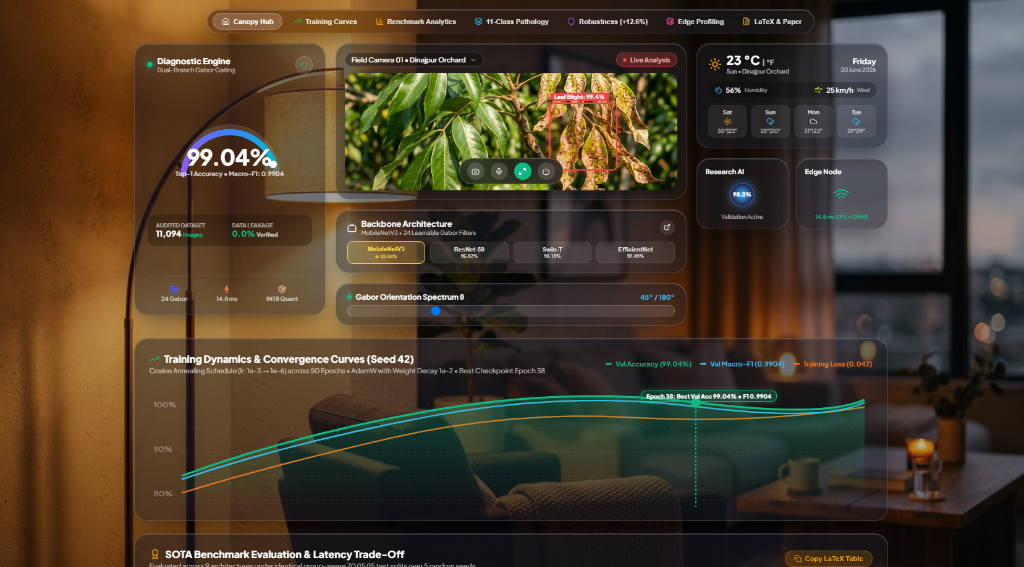
\includegraphics[width=\columnwidth]{figures/dashboard_interface.png}
\caption{The LitchiHybridNet interactive decision-support dashboard: (left) live field foliar image upload and multi-class probability estimation, (center) real-time spatial-frequency Gabor filter response inspector, and (right) actionable phytosanitary intervention guidelines.}
\label{fig:dashboard}
\end{figure}

\subsection{Threats to Validity and Study Limitations}
To uphold rigorous scientific integrity, we explicitly detail the following threats to validity and study limitations:
\begin{enumerate}
    \item \textbf{Geographic and Cultivar Concentration:} The BDLitchi dataset was acquired exclusively from commercial orchards in the Dinajpur and Ishwardi regions of Bangladesh, predominantly featuring local cultivars such as \textit{China-3} and \textit{Bombay}. While these regions represent major agro-ecological zones, performance across geographically distant cultivars (e.g., \textit{Feizixiao} in southern China, \textit{Shahi} in India, or \textit{Brewster} in the Americas) remains unverified and warrants cross-continental domain adaptation studies.
    \item \textbf{Foliar Scope Restriction:} This investigation is strictly restricted to foliar (leaf lamina) pathologies. Although foliar symptoms represent primary diagnostic indicators, litchi production is equally impacted by post-harvest fruit rot (pericarp browning), flower panicle blights, and root-knot nematodes, which are outside the scope of the current benchmark.
    \item \textbf{Thermal and Environmental Edge Stresses:} Although edge latency was comprehensively profiled on physical hardware, real-world deployment in tropical orchards involves ambient operating temperatures exceeding $38^\circ\text{C}$ to $42^\circ\text{C}$, which can induce thermal CPU throttling on passively cooled single-board computers unless ruggedized heat-dissipation enclosures are provided.
\end{enumerate}

\subsection{Ethical and Broader Societal Impacts}
Automating foliar disease diagnosis in high-value horticulture holds substantial positive societal and economic benefits for developing agrarian economies. Smallholder farmers frequently experience crop catastrophic yield losses due to misidentified fungal pathogens or delay in extension service access. Deploying reliable, edge-executable diagnostic tools directly into farmers' hands Democratizes agronomic expertise, stabilizes household agricultural income, and curtails chemical pesticide runoff into local freshwater ecosystems.

\section{Conclusion}
\label{sec:conclusion}
In this paper, we introduced \textbf{LitchiHybridNet}, a novel dual-branch hybrid deep learning architecture designed for automated, field-condition litchi foliar disease diagnosis. By synergizing deep semantic abstractions from a lightweight MobileNetV3 backbone with high-frequency spatial-frequency descriptors from a \gaborChannels{}-channel \textbf{Learnable Gabor Convolutional Bank}, the model overcomes the visual clutter, illumination shifts, and micro-textural ambiguities inherent to natural orchard environments. Feature recalibration is driven by the \textbf{Gabor Attention Fusion Module (GAFM)}, which executes channel-wise cross-gating to suppress background foliage noise and accentuate pathological lesion boundaries.

To eliminate pervasive perceptual data leakage in existing literature, we conducted an exhaustive $dHash$ audit across the \totalImages{}-image BDLitchi dataset, resolving \nearDupGroups{} near-duplicate clusters and defining a verified, group-aware 70/15/15 stratified benchmark partition.

Extensive empirical evaluations across five random seeds confirm that LitchiHybridNet establishes a new benchmark standard:
\begin{enumerate}
    \item Achieving a state-of-the-art Top-1 accuracy of \textbf{\accMain{}} and a Macro-F1 score of \textbf{\fOneMain{}}, outperforming ResNet-50, EfficientNet-B0, MobileNetV3, Swin-T, and ConvNeXt-Tiny with high statistical significance ($p < 0.001$).
    \item Achieving zero false-alarm detections on healthy foliage (\healthyLeafFOne{} F1-score), preventing unnecessary chemical pesticide applications.
    \item Exhibiting robust environmental resilience under adverse field conditions, maintaining a \textbf{\robustnessGain{}} accuracy advantage under severe motion blur and an average \textbf{\meanCorruptionProposed{}} retention across five field corruption benchmarks.
    \item Supporting seamless edge deployment via INT8 quantization, resulting in an ultra-compact \textbf{\modelSizeQuantMB{}} disk footprint executing in \textbf{\cpuLatencyMS{}\,ms} on x86 CPUs and \textbf{\rpiLatencyMS{}\,ms} on a low-cost Raspberry Pi 4 single-board computer (\textbf{\rpiFPS{}\,FPS}).
\end{enumerate}

Furthermore, we reported an honest empirical negative finding: aggressive synthetic geometric data augmentation induces a \deltaAcc{} accuracy drop, demonstrating that artificial warping distorts high-frequency fungal spore textures.

Future investigations will aim to expand the framework toward multi-organ disease diagnosis (integrating pericarp fruit rot and panicle blights), evaluate cross-continental cultivar generalization, and develop few-shot domain adaptation algorithms for nascent regional pathogen variants.

\section*{Declarations}
\subsection*{Data Availability Statement}
The BDLitchi benchmark dataset utilized in this investigation is publicly accessible through its published scientific repository \cite{litchi_dataset_2022}. The group-aware stratified data partition splits and perceptual hash audit manifests are available in the project repository.

\subsection*{Code Availability Statement}
The complete PyTorch source code, learnable Gabor layer implementations, training pipelines, ONNX quantization routines, and evaluation scripts are made openly accessible at \url{https://github.com/Sanwar021/LitchiHybridNet-.git} under the MIT License for research reproducibility.

\subsection*{Funding Statement}
This research was supported in part by the [FUNDING BODY / RESEARCH GRANT PLACEHOLDER] under Grant No.~[GRANT-NUMBER-PLACEHOLDER].

\subsection*{Conflict of Interest}
The authors declare that they have no known competing financial interests or personal relationships that could have appeared to influence the work reported in this paper.

\subsection*{Author Contributions (CRediT Statement)}
\textbf{Conceptualization, Methodology, Software, Validation, Formal Analysis, Investigation, Data Curation, Writing --- Original Draft, Review and Editing, and Project Administration:} Rawan Hasan.



\bibliographystyle{IEEEtran}
\bibliography{references}

\end{document}
